\section{Theory: derivations}
\label{app:theory}
Throughout, $z=Wf+\varepsilon$ with $f\sim\mathcal N(0,I_r)$, $\varepsilon\sim\mathcal N(0,\Psi)$, $\Psi=\mathrm{diag}(\psi)$, $W\in\mathbb R^{N\times r}$ with rows $w_j$, and parameters are known. For an observed set $S$ the posterior of $f$ given $z_S$ is Gaussian with covariance $\Sigma_S=(I+\sum_{l\in S}w_lw_l^\top/\psi_l)^{-1}$ and the posterior mean of $z_j$, $j\notin S$, has expected squared error $\psi_j+w_j^\top\Sigma_Sw_j$ (it does not depend on the observed values).

\begin{proposition}[Random subsets]\label{prop:bound}
Let $\psi_j\equiv\psi$ and let the rows $w_j$ be i.i.d.\ $\mathcal N(0,(\lambda/r)I_r)$; put $c=\lambda/(r\psi)$. For a uniformly random $S$ with $|S|=k$ and a target $j\notin S$, the relative excess error $e(k)=(\mathbb E\,\mathrm{MSE}_j-\psi)/\psi$ satisfies
\[
\frac{rc}{1+kc}\le e(k),\qquad e(k)\le \frac{r}{k-r-1}\ \ (k>r+1).
\]
\end{proposition}
\begin{proof}
$w_j$ is independent of $S$, so $\mathbb E[w_j^\top\Sigma_Sw_j]=(\lambda/r)\,\mathbb E\,\mathrm{tr}\,\Sigma_S$ and $e(k)=c\,\mathbb E\,\mathrm{tr}\,\Sigma_S$. Write $A=\sum_{l\in S}w_lw_l^\top/\psi=cQ$ with $Q\sim\mathrm{Wishart}_r(k,I)$, so $\mathbb EA=kcI$. The map $A\mapsto\mathrm{tr}(I+A)^{-1}$ is convex on positive semidefinite matrices, so Jensen gives $\mathbb E\,\mathrm{tr}(I+A)^{-1}\ge\mathrm{tr}(I+kcI)^{-1}=r/(1+kc)$, hence the lower bound. For the upper bound, $(I+A)^{-1}\preceq A^{-1}$ when $A\succ0$ ($k\ge r$), and $\mathbb E\,\mathrm{tr}\,Q^{-1}=r/(k-r-1)$ for $k>r+1$, so $\mathbb E\,\mathrm{tr}\,\Sigma_S\le r/(c(k-r-1))$ and $e(k)\le r/(k-r-1)$.
\end{proof}
Consequently a necessary condition for $e(k)\le\epsilon$ is $k\ge r/\epsilon-1/c$ and a sufficient one is $k\ge r+1+r/\epsilon$.

\begin{proposition}[Greedy information selection]\label{prop:greedy}
$F(S)=\log\det\big(I+\sum_{l\in S}v_lv_l^\top\big)$ with $v_l=w_l/\sqrt{\psi_l}$ is monotone and submodular, so greedy selection of $k$ benchmarks attains at least $(1-1/e)$ of $\max_{|S|=k}F(S)$.
\end{proposition}
\begin{proof}
With $A_S=I+\sum_{l\in S}v_lv_l^\top$ the marginal gain of $j$ is $F(S\cup j)-F(S)=\log(1+v_j^\top A_S^{-1}v_j)\ge0$. If $S\subseteq S'$ then $A_S\preceq A_{S'}$, so $A_S^{-1}\succeq A_{S'}^{-1}$ and the gain is smaller for $S'$: submodularity. The guarantee is the classical one for monotone submodular maximisation under a cardinality constraint \citep{nemhauser1978analysis}.
\end{proof}
$F(S)=2\,I(f;z_S)$ is the mutual information between the factors and the observations, which is why \texttt{dopt} targets the latent factors rather than the squared error of the targets. The error-driven rule \texttt{gv\_fa} minimises $\sum_j\mathrm{Var}(z_j\mid z_S)$ greedily; it has no submodularity guarantee in general, and its quality relative to the optimum is therefore checked by brute force on small instances (Section~\ref{sec:exp}).

\section{Additional results}
\label{app:extra}
\paragraph{Selector $\times$ inference rule.}
Table~\ref{tab:cross} gives nMSE for six selectors and five inference rules on MTEB-56 at $k=2,4,8,16$, and Table~\ref{tab:crossall} for all ten selectors (ridge and kernel ridge use the same completed training matrix; intervals are 95\% bootstrap half-widths and overlap in most cells, so compare selectors in the paired Fig.~\ref{fig:paired}). Figure~\ref{fig:allsel} shows the curves for every selector.
\begin{table}[h]
\caption{nMSE ($\pm$ half-width of the 95\% bootstrap CI over held-out models) for six selectors and five inference rules on MTEB-56 (protocol B, random 10-fold CV), at $k=2,4,8,16$. Bold: lowest point estimate in the column within each $k$.}
\label{tab:cross}
\centering\scriptsize\setlength{\tabcolsep}{3pt}
\begin{tabular}{lrrrrr}
\toprule
selector & avg-reg. & kNN & ridge & KRR & FA \\
\midrule
\multicolumn{6}{l}{\emph{$k=2$}} \\
random & 0.55\,{\scriptsize$\pm$0.08} & 0.41\,{\scriptsize$\pm$0.06} & 0.51\,{\scriptsize$\pm$0.07} & 0.41\,{\scriptsize$\pm$0.07} & 0.51\,{\scriptsize$\pm$0.07} \\
greedy cond. variance (FA) & \textbf{0.45\,{\scriptsize$\pm$0.06}} & \textbf{0.28\,{\scriptsize$\pm$0.05}} & \textbf{0.36\,{\scriptsize$\pm$0.06}} & \textbf{0.27\,{\scriptsize$\pm$0.06}} & \textbf{0.36\,{\scriptsize$\pm$0.06}} \\
greedy log-det (D-opt.) & 0.47\,{\scriptsize$\pm$0.06} & 0.34\,{\scriptsize$\pm$0.05} & 0.40\,{\scriptsize$\pm$0.05} & 0.33\,{\scriptsize$\pm$0.05} & 0.40\,{\scriptsize$\pm$0.05} \\
k-center & 0.66\,{\scriptsize$\pm$0.11} & 0.52\,{\scriptsize$\pm$0.08} & 0.57\,{\scriptsize$\pm$0.09} & 0.50\,{\scriptsize$\pm$0.08} & 0.57\,{\scriptsize$\pm$0.09} \\
leverage score & 0.74\,{\scriptsize$\pm$0.12} & 0.65\,{\scriptsize$\pm$0.10} & 0.71\,{\scriptsize$\pm$0.11} & 0.63\,{\scriptsize$\pm$0.11} & 0.71\,{\scriptsize$\pm$0.11} \\
most central & 0.46\,{\scriptsize$\pm$0.07} & 0.34\,{\scriptsize$\pm$0.05} & 0.42\,{\scriptsize$\pm$0.06} & 0.33\,{\scriptsize$\pm$0.05} & 0.42\,{\scriptsize$\pm$0.06} \\
\multicolumn{6}{l}{\emph{$k=4$}} \\
random & 0.48\,{\scriptsize$\pm$0.07} & 0.31\,{\scriptsize$\pm$0.05} & 0.37\,{\scriptsize$\pm$0.06} & 0.30\,{\scriptsize$\pm$0.06} & 0.38\,{\scriptsize$\pm$0.06} \\
greedy cond. variance (FA) & \textbf{0.41\,{\scriptsize$\pm$0.06}} & 0.25\,{\scriptsize$\pm$0.05} & 0.28\,{\scriptsize$\pm$0.06} & 0.22\,{\scriptsize$\pm$0.06} & 0.28\,{\scriptsize$\pm$0.06} \\
greedy log-det (D-opt.) & 0.41\,{\scriptsize$\pm$0.06} & \textbf{0.24\,{\scriptsize$\pm$0.04}} & \textbf{0.26\,{\scriptsize$\pm$0.04}} & \textbf{0.20\,{\scriptsize$\pm$0.03}} & \textbf{0.26\,{\scriptsize$\pm$0.04}} \\
k-center & 0.54\,{\scriptsize$\pm$0.09} & 0.34\,{\scriptsize$\pm$0.05} & 0.40\,{\scriptsize$\pm$0.05} & 0.34\,{\scriptsize$\pm$0.07} & 0.40\,{\scriptsize$\pm$0.05} \\
leverage score & 0.57\,{\scriptsize$\pm$0.08} & 0.41\,{\scriptsize$\pm$0.06} & 0.49\,{\scriptsize$\pm$0.06} & 0.38\,{\scriptsize$\pm$0.06} & 0.49\,{\scriptsize$\pm$0.06} \\
most central & 0.44\,{\scriptsize$\pm$0.06} & 0.29\,{\scriptsize$\pm$0.05} & 0.36\,{\scriptsize$\pm$0.06} & 0.28\,{\scriptsize$\pm$0.05} & 0.36\,{\scriptsize$\pm$0.06} \\
\multicolumn{6}{l}{\emph{$k=8$}} \\
random & 0.43\,{\scriptsize$\pm$0.06} & 0.26\,{\scriptsize$\pm$0.05} & 0.29\,{\scriptsize$\pm$0.05} & 0.24\,{\scriptsize$\pm$0.06} & 0.29\,{\scriptsize$\pm$0.05} \\
greedy cond. variance (FA) & 0.43\,{\scriptsize$\pm$0.06} & 0.24\,{\scriptsize$\pm$0.05} & 0.24\,{\scriptsize$\pm$0.06} & 0.20\,{\scriptsize$\pm$0.06} & 0.24\,{\scriptsize$\pm$0.06} \\
greedy log-det (D-opt.) & \textbf{0.40\,{\scriptsize$\pm$0.05}} & \textbf{0.22\,{\scriptsize$\pm$0.04}} & \textbf{0.21\,{\scriptsize$\pm$0.03}} & \textbf{0.17\,{\scriptsize$\pm$0.04}} & \textbf{0.21\,{\scriptsize$\pm$0.04}} \\
k-center & 0.46\,{\scriptsize$\pm$0.06} & 0.29\,{\scriptsize$\pm$0.05} & 0.31\,{\scriptsize$\pm$0.05} & 0.24\,{\scriptsize$\pm$0.05} & 0.32\,{\scriptsize$\pm$0.05} \\
leverage score & 0.47\,{\scriptsize$\pm$0.07} & 0.30\,{\scriptsize$\pm$0.05} & 0.33\,{\scriptsize$\pm$0.04} & 0.24\,{\scriptsize$\pm$0.04} & 0.33\,{\scriptsize$\pm$0.04} \\
most central & 0.41\,{\scriptsize$\pm$0.05} & 0.24\,{\scriptsize$\pm$0.04} & 0.24\,{\scriptsize$\pm$0.04} & 0.20\,{\scriptsize$\pm$0.04} & 0.25\,{\scriptsize$\pm$0.04} \\
\multicolumn{6}{l}{\emph{$k=16$}} \\
random & 0.41\,{\scriptsize$\pm$0.06} & 0.23\,{\scriptsize$\pm$0.04} & 0.23\,{\scriptsize$\pm$0.05} & 0.19\,{\scriptsize$\pm$0.05} & 0.23\,{\scriptsize$\pm$0.04} \\
greedy cond. variance (FA) & 0.41\,{\scriptsize$\pm$0.06} & 0.24\,{\scriptsize$\pm$0.04} & 0.21\,{\scriptsize$\pm$0.06} & 0.18\,{\scriptsize$\pm$0.06} & 0.22\,{\scriptsize$\pm$0.06} \\
greedy log-det (D-opt.) & 0.40\,{\scriptsize$\pm$0.06} & \textbf{0.21\,{\scriptsize$\pm$0.04}} & \textbf{0.20\,{\scriptsize$\pm$0.05}} & \textbf{0.16\,{\scriptsize$\pm$0.05}} & \textbf{0.19\,{\scriptsize$\pm$0.04}} \\
k-center & 0.43\,{\scriptsize$\pm$0.06} & 0.25\,{\scriptsize$\pm$0.04} & 0.23\,{\scriptsize$\pm$0.04} & 0.17\,{\scriptsize$\pm$0.04} & 0.24\,{\scriptsize$\pm$0.04} \\
leverage score & 0.42\,{\scriptsize$\pm$0.06} & 0.25\,{\scriptsize$\pm$0.04} & 0.23\,{\scriptsize$\pm$0.03} & 0.17\,{\scriptsize$\pm$0.03} & 0.24\,{\scriptsize$\pm$0.03} \\
most central & \textbf{0.40\,{\scriptsize$\pm$0.06}} & 0.22\,{\scriptsize$\pm$0.04} & 0.20\,{\scriptsize$\pm$0.04} & 0.17\,{\scriptsize$\pm$0.04} & 0.22\,{\scriptsize$\pm$0.04} \\
\bottomrule
\end{tabular}

\end{table}
\begin{table}[h]
\caption{As Table~\ref{tab:cross} for all ten selectors at $k=2,4,8,16$ (adds highest variance, most covered and conditional variance under the empirical covariance).}
\label{tab:crossall}
\centering\scriptsize\setlength{\tabcolsep}{3pt}
\begin{tabular}{lrrrrr}
\toprule
selector & avg-reg. & kNN & ridge & KRR & FA \\
\midrule
\multicolumn{6}{l}{\emph{$k=2$}} \\
random & 0.55\,{\scriptsize$\pm$0.08} & 0.41\,{\scriptsize$\pm$0.06} & 0.51\,{\scriptsize$\pm$0.07} & 0.41\,{\scriptsize$\pm$0.07} & 0.51\,{\scriptsize$\pm$0.07} \\
greedy cond. variance (FA) & \textbf{0.45\,{\scriptsize$\pm$0.06}} & \textbf{0.28\,{\scriptsize$\pm$0.05}} & \textbf{0.36\,{\scriptsize$\pm$0.06}} & \textbf{0.27\,{\scriptsize$\pm$0.06}} & \textbf{0.36\,{\scriptsize$\pm$0.06}} \\
greedy log-det (D-opt.) & 0.47\,{\scriptsize$\pm$0.06} & 0.34\,{\scriptsize$\pm$0.05} & 0.40\,{\scriptsize$\pm$0.05} & 0.33\,{\scriptsize$\pm$0.05} & 0.40\,{\scriptsize$\pm$0.05} \\
greedy cond. variance (empirical) & 0.46\,{\scriptsize$\pm$0.06} & 0.29\,{\scriptsize$\pm$0.05} & 0.37\,{\scriptsize$\pm$0.06} & 0.28\,{\scriptsize$\pm$0.06} & 0.37\,{\scriptsize$\pm$0.06} \\
k-center & 0.66\,{\scriptsize$\pm$0.11} & 0.52\,{\scriptsize$\pm$0.08} & 0.57\,{\scriptsize$\pm$0.09} & 0.50\,{\scriptsize$\pm$0.08} & 0.57\,{\scriptsize$\pm$0.09} \\
leverage score & 0.74\,{\scriptsize$\pm$0.12} & 0.65\,{\scriptsize$\pm$0.10} & 0.71\,{\scriptsize$\pm$0.11} & 0.63\,{\scriptsize$\pm$0.11} & 0.71\,{\scriptsize$\pm$0.11} \\
pivoted QR & 0.73\,{\scriptsize$\pm$0.12} & 0.64\,{\scriptsize$\pm$0.10} & 0.69\,{\scriptsize$\pm$0.11} & 0.63\,{\scriptsize$\pm$0.10} & 0.69\,{\scriptsize$\pm$0.11} \\
most central & 0.46\,{\scriptsize$\pm$0.07} & 0.34\,{\scriptsize$\pm$0.05} & 0.42\,{\scriptsize$\pm$0.06} & 0.33\,{\scriptsize$\pm$0.05} & 0.42\,{\scriptsize$\pm$0.06} \\
highest variance & 0.62\,{\scriptsize$\pm$0.11} & 0.45\,{\scriptsize$\pm$0.09} & 0.60\,{\scriptsize$\pm$0.10} & 0.45\,{\scriptsize$\pm$0.09} & 0.60\,{\scriptsize$\pm$0.10} \\
most covered & 0.59\,{\scriptsize$\pm$0.10} & 0.41\,{\scriptsize$\pm$0.08} & 0.56\,{\scriptsize$\pm$0.10} & 0.42\,{\scriptsize$\pm$0.07} & 0.56\,{\scriptsize$\pm$0.10} \\
\multicolumn{6}{l}{\emph{$k=4$}} \\
random & 0.48\,{\scriptsize$\pm$0.07} & 0.31\,{\scriptsize$\pm$0.05} & 0.37\,{\scriptsize$\pm$0.06} & 0.30\,{\scriptsize$\pm$0.06} & 0.38\,{\scriptsize$\pm$0.06} \\
greedy cond. variance (FA) & \textbf{0.41\,{\scriptsize$\pm$0.06}} & 0.25\,{\scriptsize$\pm$0.05} & 0.28\,{\scriptsize$\pm$0.06} & 0.22\,{\scriptsize$\pm$0.06} & 0.28\,{\scriptsize$\pm$0.06} \\
greedy log-det (D-opt.) & 0.41\,{\scriptsize$\pm$0.06} & \textbf{0.24\,{\scriptsize$\pm$0.04}} & \textbf{0.26\,{\scriptsize$\pm$0.04}} & \textbf{0.20\,{\scriptsize$\pm$0.03}} & \textbf{0.26\,{\scriptsize$\pm$0.04}} \\
greedy cond. variance (empirical) & 0.41\,{\scriptsize$\pm$0.06} & 0.25\,{\scriptsize$\pm$0.05} & 0.28\,{\scriptsize$\pm$0.06} & 0.23\,{\scriptsize$\pm$0.06} & 0.29\,{\scriptsize$\pm$0.06} \\
k-center & 0.54\,{\scriptsize$\pm$0.09} & 0.34\,{\scriptsize$\pm$0.05} & 0.40\,{\scriptsize$\pm$0.05} & 0.34\,{\scriptsize$\pm$0.07} & 0.40\,{\scriptsize$\pm$0.05} \\
leverage score & 0.57\,{\scriptsize$\pm$0.08} & 0.41\,{\scriptsize$\pm$0.06} & 0.49\,{\scriptsize$\pm$0.06} & 0.38\,{\scriptsize$\pm$0.06} & 0.49\,{\scriptsize$\pm$0.06} \\
pivoted QR & 0.55\,{\scriptsize$\pm$0.09} & 0.39\,{\scriptsize$\pm$0.05} & 0.47\,{\scriptsize$\pm$0.05} & 0.37\,{\scriptsize$\pm$0.06} & 0.47\,{\scriptsize$\pm$0.05} \\
most central & 0.44\,{\scriptsize$\pm$0.06} & 0.29\,{\scriptsize$\pm$0.05} & 0.36\,{\scriptsize$\pm$0.06} & 0.28\,{\scriptsize$\pm$0.05} & 0.36\,{\scriptsize$\pm$0.06} \\
highest variance & 0.59\,{\scriptsize$\pm$0.10} & 0.39\,{\scriptsize$\pm$0.07} & 0.51\,{\scriptsize$\pm$0.07} & 0.38\,{\scriptsize$\pm$0.08} & 0.51\,{\scriptsize$\pm$0.07} \\
most covered & 0.49\,{\scriptsize$\pm$0.08} & 0.33\,{\scriptsize$\pm$0.06} & 0.38\,{\scriptsize$\pm$0.06} & 0.32\,{\scriptsize$\pm$0.06} & 0.39\,{\scriptsize$\pm$0.06} \\
\multicolumn{6}{l}{\emph{$k=8$}} \\
random & 0.43\,{\scriptsize$\pm$0.06} & 0.26\,{\scriptsize$\pm$0.05} & 0.29\,{\scriptsize$\pm$0.05} & 0.24\,{\scriptsize$\pm$0.06} & 0.29\,{\scriptsize$\pm$0.05} \\
greedy cond. variance (FA) & 0.43\,{\scriptsize$\pm$0.06} & 0.24\,{\scriptsize$\pm$0.05} & 0.24\,{\scriptsize$\pm$0.06} & 0.20\,{\scriptsize$\pm$0.06} & 0.24\,{\scriptsize$\pm$0.06} \\
greedy log-det (D-opt.) & \textbf{0.40\,{\scriptsize$\pm$0.05}} & \textbf{0.22\,{\scriptsize$\pm$0.04}} & \textbf{0.21\,{\scriptsize$\pm$0.03}} & \textbf{0.17\,{\scriptsize$\pm$0.04}} & \textbf{0.21\,{\scriptsize$\pm$0.04}} \\
greedy cond. variance (empirical) & 0.43\,{\scriptsize$\pm$0.06} & 0.24\,{\scriptsize$\pm$0.05} & 0.24\,{\scriptsize$\pm$0.06} & 0.21\,{\scriptsize$\pm$0.06} & 0.25\,{\scriptsize$\pm$0.06} \\
k-center & 0.46\,{\scriptsize$\pm$0.06} & 0.29\,{\scriptsize$\pm$0.05} & 0.31\,{\scriptsize$\pm$0.05} & 0.24\,{\scriptsize$\pm$0.05} & 0.32\,{\scriptsize$\pm$0.05} \\
leverage score & 0.47\,{\scriptsize$\pm$0.07} & 0.30\,{\scriptsize$\pm$0.05} & 0.33\,{\scriptsize$\pm$0.04} & 0.24\,{\scriptsize$\pm$0.04} & 0.33\,{\scriptsize$\pm$0.04} \\
pivoted QR & 0.45\,{\scriptsize$\pm$0.06} & 0.29\,{\scriptsize$\pm$0.05} & 0.32\,{\scriptsize$\pm$0.04} & 0.24\,{\scriptsize$\pm$0.04} & 0.32\,{\scriptsize$\pm$0.04} \\
most central & 0.41\,{\scriptsize$\pm$0.05} & 0.24\,{\scriptsize$\pm$0.04} & 0.24\,{\scriptsize$\pm$0.04} & 0.20\,{\scriptsize$\pm$0.04} & 0.25\,{\scriptsize$\pm$0.04} \\
highest variance & 0.51\,{\scriptsize$\pm$0.08} & 0.29\,{\scriptsize$\pm$0.05} & 0.32\,{\scriptsize$\pm$0.06} & 0.25\,{\scriptsize$\pm$0.06} & 0.32\,{\scriptsize$\pm$0.05} \\
most covered & 0.42\,{\scriptsize$\pm$0.06} & 0.27\,{\scriptsize$\pm$0.04} & 0.27\,{\scriptsize$\pm$0.04} & 0.21\,{\scriptsize$\pm$0.03} & 0.27\,{\scriptsize$\pm$0.04} \\
\multicolumn{6}{l}{\emph{$k=16$}} \\
random & 0.41\,{\scriptsize$\pm$0.06} & 0.23\,{\scriptsize$\pm$0.04} & 0.23\,{\scriptsize$\pm$0.05} & 0.19\,{\scriptsize$\pm$0.05} & 0.23\,{\scriptsize$\pm$0.04} \\
greedy cond. variance (FA) & 0.41\,{\scriptsize$\pm$0.06} & 0.24\,{\scriptsize$\pm$0.04} & 0.21\,{\scriptsize$\pm$0.06} & 0.18\,{\scriptsize$\pm$0.06} & 0.22\,{\scriptsize$\pm$0.06} \\
greedy log-det (D-opt.) & 0.40\,{\scriptsize$\pm$0.06} & \textbf{0.21\,{\scriptsize$\pm$0.04}} & \textbf{0.20\,{\scriptsize$\pm$0.05}} & \textbf{0.16\,{\scriptsize$\pm$0.05}} & \textbf{0.19\,{\scriptsize$\pm$0.04}} \\
greedy cond. variance (empirical) & 0.41\,{\scriptsize$\pm$0.06} & 0.23\,{\scriptsize$\pm$0.04} & 0.21\,{\scriptsize$\pm$0.05} & 0.17\,{\scriptsize$\pm$0.05} & 0.22\,{\scriptsize$\pm$0.05} \\
k-center & 0.43\,{\scriptsize$\pm$0.06} & 0.25\,{\scriptsize$\pm$0.04} & 0.23\,{\scriptsize$\pm$0.04} & 0.17\,{\scriptsize$\pm$0.04} & 0.24\,{\scriptsize$\pm$0.04} \\
leverage score & 0.42\,{\scriptsize$\pm$0.06} & 0.25\,{\scriptsize$\pm$0.04} & 0.23\,{\scriptsize$\pm$0.03} & 0.17\,{\scriptsize$\pm$0.03} & 0.24\,{\scriptsize$\pm$0.03} \\
pivoted QR & 0.42\,{\scriptsize$\pm$0.06} & 0.24\,{\scriptsize$\pm$0.04} & 0.22\,{\scriptsize$\pm$0.03} & 0.17\,{\scriptsize$\pm$0.03} & 0.22\,{\scriptsize$\pm$0.03} \\
most central & \textbf{0.40\,{\scriptsize$\pm$0.06}} & 0.22\,{\scriptsize$\pm$0.04} & 0.20\,{\scriptsize$\pm$0.04} & 0.17\,{\scriptsize$\pm$0.04} & 0.22\,{\scriptsize$\pm$0.04} \\
highest variance & 0.47\,{\scriptsize$\pm$0.07} & 0.25\,{\scriptsize$\pm$0.05} & 0.26\,{\scriptsize$\pm$0.05} & 0.21\,{\scriptsize$\pm$0.06} & 0.26\,{\scriptsize$\pm$0.05} \\
most covered & 0.42\,{\scriptsize$\pm$0.06} & 0.23\,{\scriptsize$\pm$0.05} & 0.21\,{\scriptsize$\pm$0.04} & 0.18\,{\scriptsize$\pm$0.04} & 0.21\,{\scriptsize$\pm$0.03} \\
\bottomrule
\end{tabular}

\end{table}
\begin{figure}[h]
\centering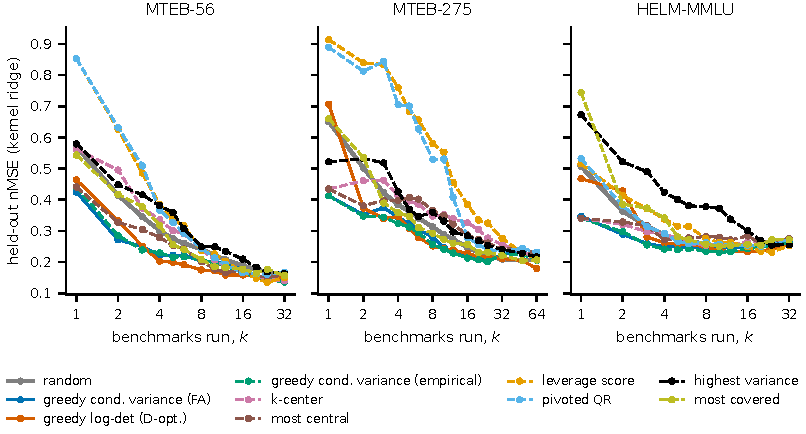
\includegraphics[width=\linewidth]{figA1_all_selectors.pdf}
\caption{Held-out nMSE against $k$ for all ten selectors (kernel ridge, protocol B) on MTEB-56, MTEB-275 and HELM-MMLU; bands are 95\% bootstrap CIs over held-out models. Leverage-score, pivoted-QR and highest-variance selection are worse than random at small $k$.}
\label{fig:allsel}
\end{figure}

\paragraph{$k^\star$ with other floors and absolute tolerances.}
Table~\ref{tab:kstar-abs} repeats Table~\ref{tab:kstar} with the floor of the best inference rule instead of the same rule ($G_{\mathrm{best}}$), and adds the smallest $k$ at which the upper confidence bound of nMSE is below an absolute tolerance. ``$>$grid'': not reached for any $k$ on the grid.
\begin{table}[h]
\caption{Smallest $k$ meeting $G_{\mathrm{best}}\ge0.8$, $0.9$ (95\% lower bound; floor = best rule) and absolute tolerances $\nmse\le0.5$, $0.25$ (95\% upper bound). Abbreviations as in Table~\ref{tab:kstar}.}
\label{tab:kstar-abs}
\centering\tiny\setlength{\tabcolsep}{2pt}
\begin{tabular}{llrrrrrrrrrrrrr}
\toprule
 & & & \multicolumn{3}{c}{$G_\mathrm{best}\geq0.8$} & \multicolumn{3}{c}{$G_\mathrm{best}\geq0.9$} & \multicolumn{3}{c}{nMSE$\leq0.5$} & \multicolumn{3}{c}{nMSE$\leq0.25$} \\
\cmidrule(lr){4-6}\cmidrule(lr){7-9}\cmidrule(lr){10-12}\cmidrule(lr){13-15}
dataset & rule & floor & rand. & GV & D-opt & rand. & GV & D-opt & rand. & GV & D-opt & rand. & GV & D-opt \\
\midrule
mteb-dense56 & krr & 0.15 & 5 & 2 & 3 & 12 & 8 & 4 & 2 & 1 & 2 & 16 & 16 & 4 \\
mteb-dense56 & fa & 0.18 & 8 & 5 & 4 & 24 & 20 & 10 & 3 & 2 & 2 & 32 & 32 & 16 \\
mteb-dense & krr & 0.32 & 8 & 8 & 6 & 20 & 12 & 16 & 3 & 1 & 2 & 32 & 24 & 64 \\
mteb-dense & fa & 0.18 & 10 & 6 & 8 & 32 & 16 & 20 & 4 & 2 & 3 & 48 & 64 & 32 \\
mteb-mid & krr & 0.35 & 10 & 6 & 6 & 20 & 16 & 16 & 3 & 2 & 2 & $>$grid & 24 & 24 \\
mteb-mid & fa & 0.17 & 16 & 8 & 12 & 48 & 24 & 32 & 5 & 3 & 5 & 64 & 48 & 48 \\
mteb-sparse & krr & 0.43 & 10 & 12 & 12 & 48 & $>$grid & $>$grid & 5 & 2 & 4 & $>$grid & $>$grid & $>$grid \\
mteb-sparse & fa & 0.18 & 16 & 16 & 24 & 48 & 32 & 24 & 6 & 5 & 8 & 48 & $>$grid & $>$grid \\
helm-mmlu & krr & 0.28 & 2 & 1 & 3 & 4 & 2 & 3 & 4 & 2 & 3 & $>$grid & $>$grid & $>$grid \\
helm-mmlu & fa & 0.21 & 3 & 1 & 3 & 5 & 3 & 4 & 4 & 3 & 4 & $>$grid & $>$grid & $>$grid \\
helm & krr & 0.26 & 4 & 2 & 2 & 6 & 3 & 5 & 4 & 2 & 2 & $>$grid & $>$grid & $>$grid \\
helm & fa & 0.36 & $>$grid & 4 & 5 & $>$grid & $>$grid & $>$grid & $>$grid & 2 & 2 & $>$grid & $>$grid & $>$grid \\
helm-lite-ext & krr & 0.35 & 6 & 3 & 4 & 12 & 4 & 4 & 8 & 3 & 4 & $>$grid & $>$grid & $>$grid \\
helm-lite-ext & fa & 0.31 & 8 & 3 & 4 & 12 & 5 & 5 & 10 & 3 & 4 & $>$grid & $>$grid & $>$grid \\
livebench & krr & 0.34 & 2 & 2 & 1 & 2 & 4 & 2 & 1 & 1 & 1 & $>$grid & $>$grid & $>$grid \\
livebench & fa & 0.32 & 2 & 2 & 2 & 3 & 3 & 2 & 2 & 2 & 2 & $>$grid & $>$grid & $>$grid \\
olb & krr & 0.29 & 2 & 1 & 1 & $>$grid & $>$grid & $>$grid & 2 & 1 & 1 & $>$grid & $>$grid & $>$grid \\
olb & fa & 0.34 & 3 & 2 & 2 & $>$grid & $>$grid & $>$grid & 2 & 1 & 1 & $>$grid & $>$grid & $>$grid \\
\bottomrule
\end{tabular}

\end{table}

\paragraph{Matrices.}
\begin{table}[h]
\caption{Score matrices (models $M$ $\times$ benchmarks $N$). \emph{PR rank}: participation-ratio effective rank of the standardised matrix; \emph{FA rank (CV)}: rank chosen by hold-out error; \emph{noise nMSE}: mean measurement-noise variance on the cells with repeated runs, in units of the benchmark variance (a lower bound on unavoidable error, available only for the $18\%$ ($28\%$) of cells of MTEB-56 (MTEB-275) with repeat runs). Generated by \texttt{code/figtab/tables.py} from \texttt{results/summary/datasets.csv}.}
\label{tab:data}
\centering\small\setlength{\tabcolsep}{3.5pt}
\begin{tabular}{lrrrrrrrr}
\toprule
dataset & $M$ & $N$ & obs.\ \% & PC1 \% & PCs 80/90\% & PR rank & FA rank (CV) & noise nMSE \\
\midrule
mteb-dense56 & 152 & 56 & 99.6 & 63 & 3 / 9 & 2.4 & 12 & 0.028 \\
mteb-dense & 133 & 275 & 98.9 & 54 & 7 / 17 & 3.2 & 16 & 0.060 \\
mteb-mid & 156 & 357 & 92.1 & 54 & 8 / 19 & 3.2 & 24 & -- \\
mteb-sparse & 479 & 472 & 30.2 & 36 & 19 / 43 & 6.8 & 16 & -- \\
helm-mmlu & 79 & 57 & 100.0 & 80 & 2 / 4 & 1.6 & 3 & -- \\
helm & 91 & 10 & 99.9 & 63 & 2 / 4 & 2.3 & 3 & -- \\
helm-lite-ext & 91 & 28 & 99.9 & 61 & 4 / 8 & 2.6 & 6 & -- \\
livebench & 195 & 7 & 76.7 & 62 & 3 / 4 & 2.4 & 2 & -- \\
olb & 4497 & 6 & 100.0 & 74 & 2 / 3 & 1.8 & 2 & -- \\
\bottomrule
\end{tabular}

\end{table}
\begin{figure}[h]
\centering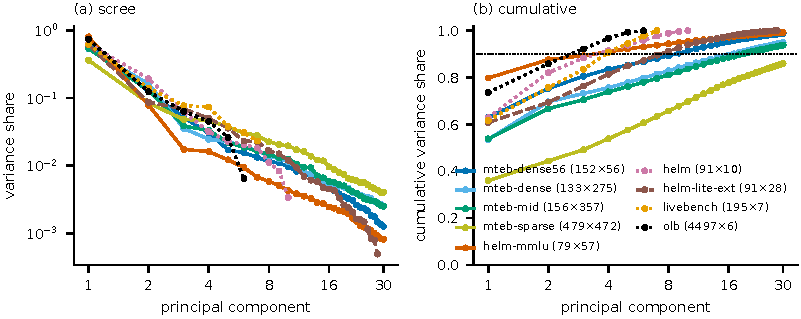
\includegraphics[width=0.85\linewidth]{fig2_scree.pdf}
\caption{Spectrum of each standardised real score matrix (PCA on the completed matrix): (a) variance share per principal component, (b) cumulative share, dotted line $90\%$.}
\label{fig:scree}
\end{figure}
\begin{figure}[h]
\centering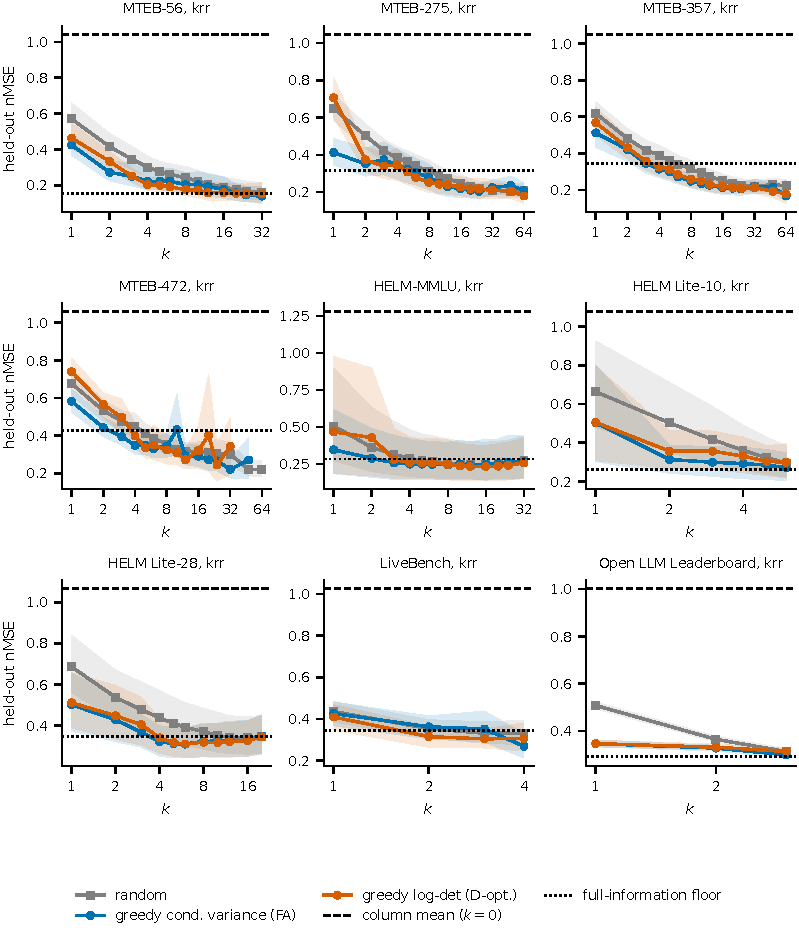
\includegraphics[width=\linewidth]{fig4b_datasets.pdf}
\caption{The comparison of Fig.~\ref{fig:main} on every real matrix (protocol B, random folds): random selection against greedy conditional variance and greedy log-det; $k$ axes differ because $N$ ranges from $6$ to $472$.}
\label{fig:datasets}
\end{figure}

\paragraph{Oracle, leakage and cost.}
Table~\ref{tab:oracle} compares random, the two deployable greedy selectors and the oracle (which uses the held-out model's own target scores and is therefore an optimistic bound) on four matrices. The oracle is clearly better only at $k\le2$ on MTEB-56 ($0.23$ against $0.27$ and $0.33$ at $k=2$) and on HELM Lite and the Open LLM Leaderboard ($k=2$: $0.19$ and $0.22$ against $0.31$--$0.36$); at $k=4$ and $8$ on MTEB-56 it is within the confidence intervals of log-det selection. Table~\ref{tab:leak} lists the leakage check of Fig.~\ref{fig:oracle}b by $k$.
\begin{table}[h]
\caption{Oracle selection against random and deployable greedy selectors (kernel ridge; nMSE $\pm$ half-width of the 95\% CI; GV: greedy conditional variance; ``--'': $k$ outside the dataset's grid).}
\label{tab:oracle}
\centering\scriptsize\setlength{\tabcolsep}{3pt}
\begin{tabular}{lrrrrr}
\toprule
dataset & $k$ & random & GV & D-opt & oracle \\
\midrule
mteb-dense56 & 2 & 0.41\,{\scriptsize$\pm$0.07} & 0.27\,{\scriptsize$\pm$0.06} & 0.33\,{\scriptsize$\pm$0.05} & 0.23\,{\scriptsize$\pm$0.03} \\
 & 4 & 0.30\,{\scriptsize$\pm$0.06} & 0.22\,{\scriptsize$\pm$0.06} & 0.20\,{\scriptsize$\pm$0.03} & 0.19\,{\scriptsize$\pm$0.03} \\
 & 8 & 0.24\,{\scriptsize$\pm$0.06} & 0.20\,{\scriptsize$\pm$0.06} & 0.17\,{\scriptsize$\pm$0.04} & 0.15\,{\scriptsize$\pm$0.03} \\
\midrule
helm-mmlu & 2 & 0.36\,{\scriptsize$\pm$0.22} & 0.29\,{\scriptsize$\pm$0.16} & 0.43\,{\scriptsize$\pm$0.36} & 0.29\,{\scriptsize$\pm$0.18} \\
 & 4 & 0.29\,{\scriptsize$\pm$0.16} & 0.25\,{\scriptsize$\pm$0.14} & 0.26\,{\scriptsize$\pm$0.14} & 0.22\,{\scriptsize$\pm$0.12} \\
 & 8 & 0.26\,{\scriptsize$\pm$0.13} & 0.24\,{\scriptsize$\pm$0.13} & 0.25\,{\scriptsize$\pm$0.13} & 0.18\,{\scriptsize$\pm$0.10} \\
\midrule
helm & 2 & 0.50\,{\scriptsize$\pm$0.18} & 0.31\,{\scriptsize$\pm$0.07} & 0.36\,{\scriptsize$\pm$0.10} & 0.19\,{\scriptsize$\pm$0.05} \\
 & 4 & 0.36\,{\scriptsize$\pm$0.12} & 0.29\,{\scriptsize$\pm$0.08} & 0.33\,{\scriptsize$\pm$0.09} & 0.18\,{\scriptsize$\pm$0.06} \\
 & 8 & -- & -- & -- & -- \\
\midrule
livebench & 2 & 0.35\,{\scriptsize$\pm$0.04} & 0.36\,{\scriptsize$\pm$0.06} & 0.32\,{\scriptsize$\pm$0.05} & 0.21\,{\scriptsize$\pm$0.03} \\
 & 4 & 0.33\,{\scriptsize$\pm$0.06} & 0.27\,{\scriptsize$\pm$0.06} & 0.31\,{\scriptsize$\pm$0.07} & 0.31\,{\scriptsize$\pm$0.06} \\
 & 8 & -- & -- & -- & -- \\
\midrule
olb & 2 & 0.36\,{\scriptsize$\pm$0.01} & 0.32\,{\scriptsize$\pm$0.01} & 0.32\,{\scriptsize$\pm$0.02} & 0.22\,{\scriptsize$\pm$0.01} \\
 & 4 & -- & -- & -- & -- \\
 & 8 & -- & -- & -- & -- \\
\bottomrule
\end{tabular}

\end{table}
\begin{table}[h]
\caption{Leakage check (kernel ridge, nMSE): selection model fitted on training models only / also on the held-out rows. Random selection is identical by construction.}
\label{tab:leak}
\centering\scriptsize\setlength{\tabcolsep}{3pt}
\begin{tabular}{llrrrr}
\toprule
dataset & selector & $k=2$ & $k=4$ & $k=8$ & $k=16$ \\
\midrule
mteb-dense56 & random & 0.415 / 0.415 & 0.301 / 0.301 & 0.241 / 0.241 & 0.188 / 0.188 \\
mteb-dense56 & greedy cond. variance (FA) & 0.271 / 0.269 & 0.222 / 0.190 & 0.203 / 0.195 & 0.176 / 0.168 \\
mteb-dense56 & greedy log-det (D-opt.) & 0.333 / 0.334 & 0.203 / 0.204 & 0.175 / 0.166 & 0.159 / 0.131 \\
helm-mmlu & random & 0.363 / 0.363 & 0.287 / 0.287 & 0.257 / 0.257 & 0.246 / 0.246 \\
helm-mmlu & greedy cond. variance (FA) & 0.289 / 0.297 & 0.250 / 0.238 & 0.245 / 0.236 & 0.249 / 0.244 \\
helm-mmlu & greedy log-det (D-opt.) & 0.428 / 0.330 & 0.262 / 0.236 & 0.248 / 0.228 & 0.234 / 0.234 \\
\bottomrule
\end{tabular}

\end{table}
\begin{figure}[h]
\centering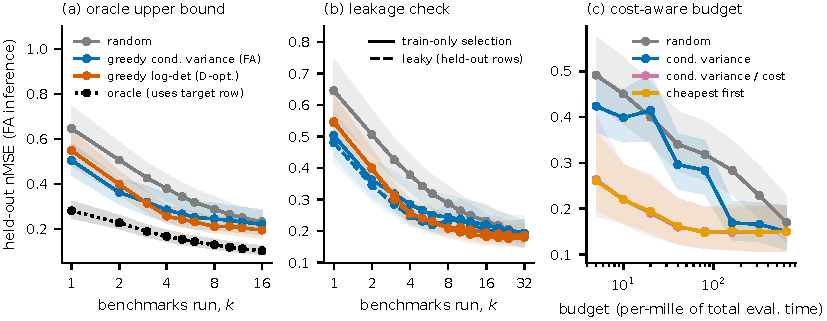
\includegraphics[width=\linewidth]{figA2_oracle_leak_cost.pdf}
\caption{MTEB-56. (a) Oracle selection, which uses the held-out model's own target scores (optimistic upper bound, not a method). (b) Leakage check: the selection model fitted on training models only (solid, used everywhere) against also on the held-out rows (dashed). Panels (a, b) use factor-analysis inference, panel (c) kernel ridge; the text and Tables~\ref{tab:oracle}, \ref{tab:leak} give kernel ridge. (c) Cost-aware selection: the budget is a share, in per mille, of the total evaluation time of the candidate tasks.}
\label{fig:oracle}
\end{figure}
Cost-aware selection (greedy conditional variance per unit cost, and a cheapest-first rule) reaches $\nmse=0.26$ with kernel ridge at a budget of $5$\textperthousand\ of the total evaluation time of the 56 tasks, against $0.49$ for random tasks and $0.42$ for cost-blind conditional variance, which pays for expensive tasks first; at $20$\textperthousand\ the values are $0.19$ (cost-aware), $0.40$ (random) and $0.42$ (cost-blind). This holds on MTEB-56 only: on MTEB-275 the cost-aware rules are good at $5$--$10$\textperthousand\ ($0.20$--$0.23$ against $0.26$--$0.37$ for cost-blind and $0.34$--$0.39$ for random) but at $20$\textperthousand\ they are \emph{worse than random} ($0.75$ and $1.24$ against $0.29$), and from $160$\textperthousand\ they stay above both other rules ($0.34$ against $0.26$ and $0.25$) until the budget reaches $640$\textperthousand\ ($0.32$ against $0.56$ and $0.43$). We therefore do not claim a general result for cost-aware selection and did not investigate the cause. Task costs are the median evaluation time per task from the result files, a coarse proxy.

\begin{figure}[h]
\centering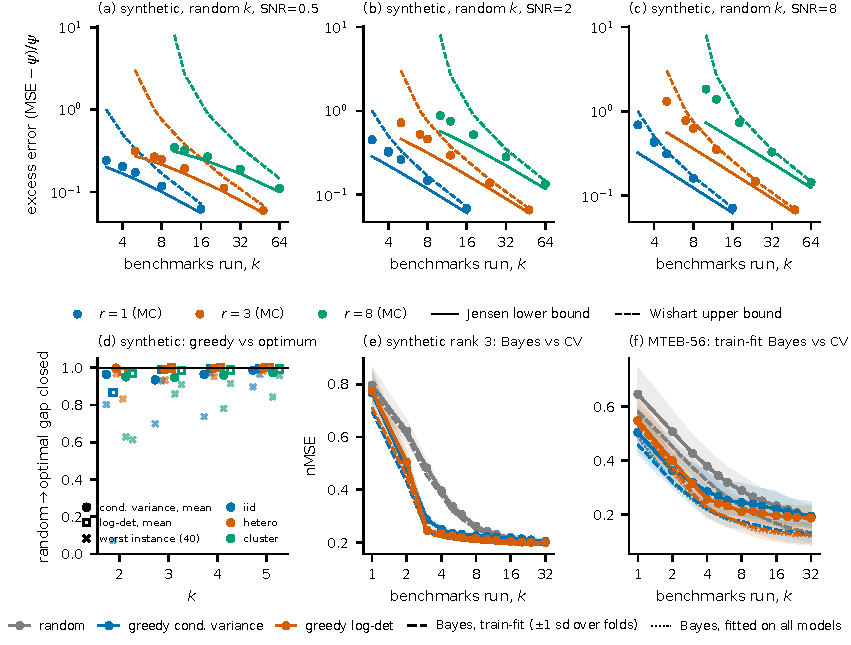
\includegraphics[width=0.85\linewidth]{fig6_theory.pdf}
\caption{(a--c) Synthetic matrices with known truth: excess error over the noise floor for random $k$ under Bayes-optimal inference (Monte Carlo) with the lower and upper bounds of Proposition~\ref{prop:bound}. (d) Synthetic, $N=16$: fraction of the random-to-optimal gap closed by the greedy rules (mean over 40 matrices, worst matrix). (e, f) Model-implied (dashed) and cross-validated (solid) nMSE for a synthetic rank-3 matrix and for MTEB-56; for MTEB-56 the dashed curve uses a covariance fitted on each fold's training models only (band: $\pm1$ sd of the model-implied error over folds), and the dotted curve the earlier in-sample fit, which is optimistic.}
\label{fig:theory}
\end{figure}
\paragraph{Synthetic data conditions.}
Table~\ref{tab:syn} shows selection on synthetic rank-$r$ matrices with known structure (factor-analysis inference; these are controlled checks and not evidence about any real leaderboard). Informed selection beats random selection in every condition at $k\le4$ (e.g.\ $0.25$ and $0.23$ against $0.40$ on the base matrix at $k=4$); the gain is smaller with high noise ($0.66\to0.51$, $k=4$), with rank $8$ ($0.68\to0.58$--$0.63$, $k=4$), and with correlated benchmark clusters at $k=8$ ($0.42\to0.38$--$0.40$), and with $M=30$ training models the errors are higher throughout.
\begin{table}[h]
\caption{SYNTHETIC matrices only: nMSE of the column mean and of random, greedy conditional-variance (GV) and greedy log-det (D-opt) selection with factor-analysis inference (base: rank 3; noisy; clustered; heterogeneous; rank 8; $M=30$ training models).}
\label{tab:syn}
\centering\scriptsize\setlength{\tabcolsep}{3pt}
\begin{tabular}{lrrrrr}
\toprule
SYNTHETIC matrix & $k$ & col.\ mean & random & GV & D-opt \\
\midrule
syn.\ M30 & 2 & 1.15 & 0.75\,{\scriptsize$\pm$0.14} & 0.50\,{\scriptsize$\pm$0.13} & 0.50\,{\scriptsize$\pm$0.13} \\
 & 4 & 1.15 & 0.52\,{\scriptsize$\pm$0.08} & 0.36\,{\scriptsize$\pm$0.05} & 0.34\,{\scriptsize$\pm$0.04} \\
 & 8 & 1.15 & 0.38\,{\scriptsize$\pm$0.04} & 0.35\,{\scriptsize$\pm$0.05} & 0.32\,{\scriptsize$\pm$0.04} \\
\midrule
syn.\ base & 2 & 1.03 & 0.62\,{\scriptsize$\pm$0.04} & 0.48\,{\scriptsize$\pm$0.05} & 0.50\,{\scriptsize$\pm$0.05} \\
 & 4 & 1.03 & 0.40\,{\scriptsize$\pm$0.02} & 0.25\,{\scriptsize$\pm$0.01} & 0.23\,{\scriptsize$\pm$0.01} \\
 & 8 & 1.03 & 0.26\,{\scriptsize$\pm$0.01} & 0.23\,{\scriptsize$\pm$0.01} & 0.22\,{\scriptsize$\pm$0.01} \\
\midrule
syn.\ clust & 2 & 1.03 & 0.70\,{\scriptsize$\pm$0.06} & 0.44\,{\scriptsize$\pm$0.02} & 0.46\,{\scriptsize$\pm$0.03} \\
 & 4 & 1.03 & 0.52\,{\scriptsize$\pm$0.03} & 0.41\,{\scriptsize$\pm$0.02} & 0.42\,{\scriptsize$\pm$0.02} \\
 & 8 & 1.03 & 0.42\,{\scriptsize$\pm$0.02} & 0.40\,{\scriptsize$\pm$0.02} & 0.38\,{\scriptsize$\pm$0.02} \\
\midrule
syn.\ hetero & 2 & 1.03 & 0.78\,{\scriptsize$\pm$0.07} & 0.58\,{\scriptsize$\pm$0.05} & 0.66\,{\scriptsize$\pm$0.08} \\
 & 4 & 1.03 & 0.60\,{\scriptsize$\pm$0.04} & 0.38\,{\scriptsize$\pm$0.02} & 0.37\,{\scriptsize$\pm$0.02} \\
 & 8 & 1.03 & 0.45\,{\scriptsize$\pm$0.02} & 0.38\,{\scriptsize$\pm$0.02} & 0.37\,{\scriptsize$\pm$0.02} \\
\midrule
syn.\ miss50 & 2 & 1.07 & 0.65\,{\scriptsize$\pm$0.06} & 0.64\,{\scriptsize$\pm$0.08} & 0.54\,{\scriptsize$\pm$0.07} \\
 & 4 & 1.07 & 0.42\,{\scriptsize$\pm$0.03} & 0.49\,{\scriptsize$\pm$0.06} & 0.30\,{\scriptsize$\pm$0.02} \\
 & 8 & 1.07 & 0.29\,{\scriptsize$\pm$0.02} & 0.33\,{\scriptsize$\pm$0.03} & 0.26\,{\scriptsize$\pm$0.02} \\
\midrule
syn.\ noisy & 2 & 1.03 & 0.79\,{\scriptsize$\pm$0.05} & 0.68\,{\scriptsize$\pm$0.05} & 0.66\,{\scriptsize$\pm$0.05} \\
 & 4 & 1.03 & 0.66\,{\scriptsize$\pm$0.03} & 0.51\,{\scriptsize$\pm$0.02} & 0.51\,{\scriptsize$\pm$0.03} \\
 & 8 & 1.03 & 0.53\,{\scriptsize$\pm$0.02} & 0.49\,{\scriptsize$\pm$0.02} & 0.47\,{\scriptsize$\pm$0.02} \\
\midrule
syn.\ r8 & 2 & 1.03 & 0.85\,{\scriptsize$\pm$0.07} & 0.82\,{\scriptsize$\pm$0.07} & 0.83\,{\scriptsize$\pm$0.08} \\
 & 4 & 1.03 & 0.68\,{\scriptsize$\pm$0.05} & 0.63\,{\scriptsize$\pm$0.06} & 0.58\,{\scriptsize$\pm$0.05} \\
 & 8 & 1.03 & 0.42\,{\scriptsize$\pm$0.02} & 0.28\,{\scriptsize$\pm$0.01} & 0.27\,{\scriptsize$\pm$0.02} \\
\bottomrule
\end{tabular}

\end{table}

\begin{figure}[h]
\centering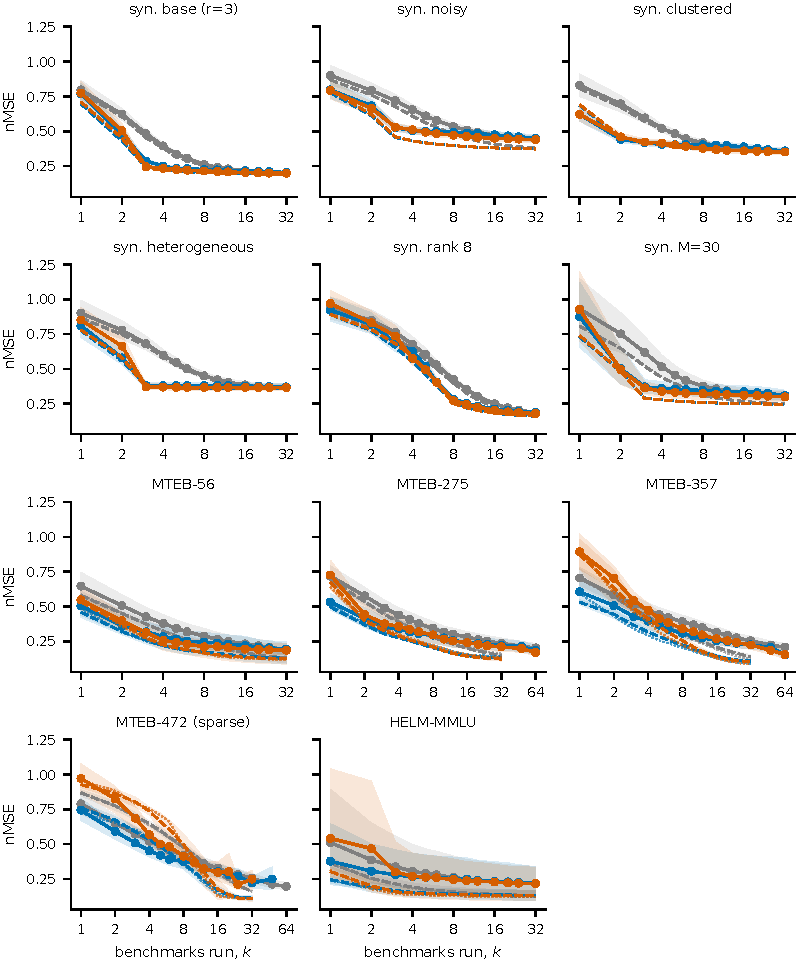
\includegraphics[width=\linewidth]{figA3_theory_vs_cv_all.pdf}
\caption{Panels (e, f) of Fig.~\ref{fig:theory} for every matrix with a model-implied curve (synthetic matrices are marked ``syn.''); real matrices: dashed, covariance fitted on training folds ($\pm1$ sd over folds); dotted, in-sample fit.}
\label{fig:theorycv}
\end{figure}

\paragraph{Missingness, training-set size and rank.} Fig.~\ref{fig:cond} shows the sensitivity analyses described in Section~\ref{sec:exp}.
\begin{figure}[t]
\centering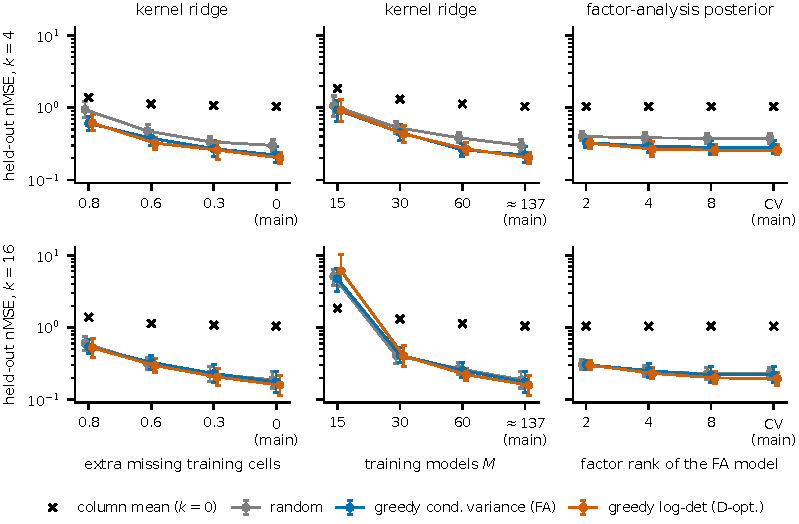
\includegraphics[width=0.68\linewidth]{fig4_conditions.pdf}
\caption{Sensitivity on MTEB-56 at $k=4$ (top) and $k=16$ (bottom): extra missing-at-random training cells, number of training models $M$, and fixed factor rank. Crosses: column-mean error under the same condition; bars: 95\% bootstrap CI.}
\label{fig:cond}
\end{figure}
\paragraph{Dependence-robust intervals and $k^\star$ by split.} The main intervals bootstrap held-out models. We also resampled organisations and strict model families (union of organisations that share a model family; the HELM organisation is a name-derived proxy), $1000$ resamples, on the three MTEB blocks and HELM-MMLU (\texttt{cluster\_*.csv}). Fig.~\ref{fig:clpaired} compares the two intervals for the paired contrasts; family-clustered intervals are $0.46$--$2.53$ times as wide as the model-level ones (median $1.11$ over the plotted contrasts), keep the sign of conditional variance and log-det against random almost everywhere and weaken the case for centrality against random (on MTEB-56 only $k=1$ remains separated from zero for $k\le8$; $k=2$: $[-0.133,0.003]$, $k=8$: $[-0.066,0.015]$). Table~\ref{tab:kstarcl} gives $k^\star$ under both schemes and its variation across repetitions (the entry for conditional variance with the factor posterior at $g=0.9$ is $20$ here and $16$ in Table~\ref{tab:kstar} on MTEB-56 and MTEB-275: the lower bound of $G$ grazes $0.9$ over several $k$, so this value moves with the resampling seed; random with the factor posterior at $g=0.9$ on MTEB-357 is ``$>$grid'' here, the grid ending at $32$, against $48$ in Table~\ref{tab:kstar}); Table~\ref{tab:kstarsplit} gives $k^\star$ under organisation, strict-family and temporal splits. Leave-organisation-out leaves no held-out model with two same-organisation models in training, but $47\%$ (MTEB-56) and $52\%$ (MTEB-275) still have two same-family models; strict-family leave-out removes both (\texttt{group\_counts.csv}).
\begin{figure}[h]
\centering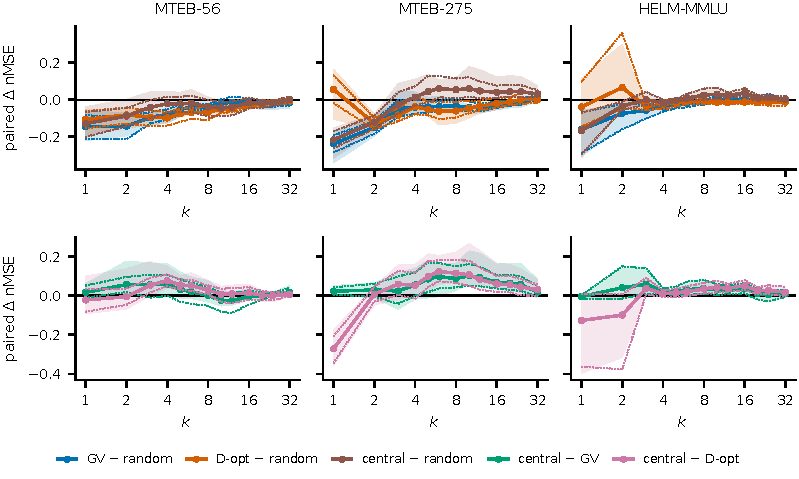
\includegraphics[width=\linewidth]{figA4_cluster_paired.pdf}
\caption{Paired differences in nMSE between selectors (kernel ridge, random folds; columns: MTEB-56, MTEB-275, HELM-MMLU; below $0$ favours the first-named selector; top: conditional variance, log-det and central against random, bottom: central against conditional variance and log-det). Shaded: 95\% CI from a bootstrap over strict families; dotted: bootstrap over models (same 1000 resamples).}
\label{fig:clpaired}
\end{figure}
\begin{table}[h]
\caption{$k^\star(g)$ with the CI taken from the bootstrap over models / over strict families (kernel ridge and factor posterior; $>$32: not reached on the grid), and the range of the point $k^\star$ over the repetitions (fold-assignment draws). ``central'': most-central selection.}
\label{tab:kstarcl}
\centering\tiny\setlength{\tabcolsep}{2pt}
\begin{tabular}{llrrrrrrrrr}
\toprule
 & & & \multicolumn{4}{c}{$k^\star$ (CI rule): model / family} & \multicolumn{4}{c}{point $k^\star$ over repetitions} \\
\cmidrule(lr){4-7}\cmidrule(lr){8-11}
dataset & rule & $g$ & rand. & GV & D-opt & central & rand. & GV & D-opt & central \\
\midrule
mteb-dense56 & krr & 0.8 & 5/5 & 2/3 & 3/3 & 4/5 & 4 & 2 & 2--3 & 2--3 \\
 & krr & 0.9 & 12/12 & 8/8 & 4/6 & 10/10 & 8--10 & 3--8 & 3--4 & 5--8 \\
 & fa & 0.8 & 8/8 & 4/4 & 3/4 & 6/6 & 5--6 & 2--3 & 3 & 4--5 \\
 & fa & 0.9 & 16/16 & 20/10 & 5/6 & 10/12 & 10--12 & 4--12 & 4--6 & 8 \\
\midrule
mteb-dense & krr & 0.8 & 3/3 & 1/1 & 2/2 & 2/2 & 3 & 1 & 2 & 1 \\
 & krr & 0.9 & 6/6 & 5/5 & 3/4 & 12/16 & 4 & 2 & 2 & 2 \\
 & fa & 0.8 & 10/10 & 6/8 & 8/8 & 24/32 & 8 & 3 & 4--5 & 12--20 \\
 & fa & 0.9 & 32/32 & 20/16 & 20/16 & $>$32/$>$32 & 20--24 & 12 & 10--12 & 32 \\
\midrule
mteb-mid & krr & 0.8 & 3/3 & 2/3 & 2/2 & 5/6 & 2--3 & 2 & 2 & 2--3 \\
 & krr & 0.9 & 5/4 & 3/3 & 3/3 & 8/10 & 3--5 & 2--3 & 2--3 & 3--6 \\
 & fa & 0.8 & 16/16 & 8/8 & 12/10 & $>$32/$>$32 & 12--16 & 6 & 8--10 & $>$32 \\
 & fa & 0.9 & $>$32/$>$32 & 24/32 & 32/32 & $>$32/$>$32 & 32 & 16--24 & 20 & $>$32 \\
\midrule
mteb-sparse & krr & 0.8 & 3/3 & 2/2 & 4/4 & 4/4 & 1--5 & 1--3 & 2--4 & 1--24 \\
 & krr & 0.9 & 5/5 & 3/3 & 4/4 & $>$32/16 & 2--10 & 1--4 & 2--5 & 1 \\
 & fa & 0.8 & 16/16 & 16/16 & 16/24 & $>$32/$>$32 & 12--16 & 8--12 & 12 & $>$32 \\
 & fa & 0.9 & $>$32/$>$32 & $>$32/32 & 24/24 & $>$32/$>$32 & 32 & 20--32 & 20--24 & $>$32 \\
\midrule
helm-mmlu & krr & 0.8 & 2/2 & 1/1 & 3/3 & 1/1 & 1--2 & 1 & 1--3 & 1 \\
 & krr & 0.9 & 3/2 & 1/1 & 3/3 & 1/1 & 1--3 & 1--2 & 1--3 & 1 \\
 & fa & 0.8 & 3/3 & 1/2 & 3/3 & 1/1 & 2--3 & 1 & 1--3 & 1 \\
 & fa & 0.9 & 5/5 & 3/3 & 4/4 & 16/16 & 3--5 & 2--3 & 3--4 & 1--4 \\
\bottomrule
\end{tabular}

\end{table}
\begin{table}[h]
\caption{$k^\star(G\ge0.8)$ by selector (kernel ridge and factor posterior). Random folds: CI rule with the bootstrap over models, organisations or strict families (1000 resamples), each with the $[2.5,97.5]\%$ range of the point $k^\star$ over the resamples. Right: the same criterion (bootstrap over models) under leave-organisation-out, strict-family leave-out and the temporal split (single fold, MTEB only). ``--'': selector not run on that split. Under shift the floor and the column mean are far higher (temporal MTEB-56: $1.4$--$1.5$ and $4.6$), so $G$ is relative to a poor floor.}
\label{tab:kstarsplit}
\centering\scriptsize\setlength{\tabcolsep}{3pt}
\begin{tabular}{lllcccrrr}
\toprule
 & & & \multicolumn{3}{c}{random folds: $k^\star$ [95\% interval of point $k^\star$]} & \multicolumn{3}{c}{shift splits} \\
\cmidrule(lr){4-6}\cmidrule(lr){7-9}
matrix & rule & selector & model CI & org. CI & family CI & org. out & family out & temporal \\
\midrule
MTEB-56 & krr & random & 5 {\scriptsize[3--5]} & 5 {\scriptsize[3--5]} & 5 {\scriptsize[3--5]} & 6 & 6 & 6 \\
 &  & GV & 2 {\scriptsize[2--2]} & 3 {\scriptsize[1--3]} & 3 {\scriptsize[2--3]} & 8 & 2 & 4 \\
 &  & D-opt & 3 {\scriptsize[2--3]} & 3 {\scriptsize[2--3]} & 3 {\scriptsize[2--3]} & 3 & 8 & 2 \\
 &  & central & 4 {\scriptsize[2--4]} & 5 {\scriptsize[2--5]} & 5 {\scriptsize[2--5]} & -- & 10 & -- \\
\cmidrule(lr){2-9}
 & fa & random & 8 {\scriptsize[4--8]} & 8 {\scriptsize[4--8]} & 8 {\scriptsize[4--8]} & 8 & 8 & 5 \\
 &  & GV & 4 {\scriptsize[2--4]} & 5 {\scriptsize[2--5]} & 4 {\scriptsize[2--4]} & 16 & 5 & 4 \\
 &  & D-opt & 3 {\scriptsize[3--3]} & 4 {\scriptsize[2--4]} & 4 {\scriptsize[2--4]} & 4 & 6 & 2 \\
 &  & central & 6 {\scriptsize[3--6]} & 6 {\scriptsize[3--6]} & 6 {\scriptsize[3--6]} & -- & 10 & -- \\
\midrule
MTEB-275 & krr & random & 3 {\scriptsize[3--3]} & 4 {\scriptsize[2--4]} & 3 {\scriptsize[2--3]} & 4 & 3 & 6 \\
 &  & GV & 1 {\scriptsize[1--1]} & 2 {\scriptsize[1--2]} & 1 {\scriptsize[1--1]} & 5 & 1 & 4 \\
 &  & D-opt & 2 {\scriptsize[2--2]} & 2 {\scriptsize[2--2]} & 2 {\scriptsize[2--2]} & -- & 2 & -- \\
 &  & central & 2 {\scriptsize[1--2]} & 2 {\scriptsize[1--2]} & 2 {\scriptsize[1--2]} & -- & 1 & -- \\
\cmidrule(lr){2-9}
 & fa & random & 10 {\scriptsize[6--10]} & 10 {\scriptsize[6--10]} & 10 {\scriptsize[6--10]} & 10 & 8 & 16 \\
 &  & GV & 6 {\scriptsize[3--6]} & 6 {\scriptsize[3--6]} & 8 {\scriptsize[2--8]} & 6 & 5 & 8 \\
 &  & D-opt & 8 {\scriptsize[3--8]} & 8 {\scriptsize[3--8]} & 8 {\scriptsize[3--8]} & -- & 3 & -- \\
 &  & central & 24 {\scriptsize[10--24]} & 24 {\scriptsize[10--24]} & 32 {\scriptsize[10--32]} & -- & 20 & -- \\
\midrule
MTEB-472 & krr & random & 3 {\scriptsize[2--3]} & 4 {\scriptsize[2--4]} & 3 {\scriptsize[1--3]} & -- & -- & -- \\
 &  & GV & 2 {\scriptsize[1--2]} & 2 {\scriptsize[1--2]} & 2 {\scriptsize[1--2]} & -- & -- & -- \\
 &  & D-opt & 4 {\scriptsize[2--4]} & 4 {\scriptsize[2--4]} & 4 {\scriptsize[1--4]} & -- & -- & -- \\
 &  & central & 4 {\scriptsize[1--4]} & 4 {\scriptsize[1--4]} & 4 {\scriptsize[1--4]} & -- & -- & -- \\
\cmidrule(lr){2-9}
 & fa & random & 16 {\scriptsize[12--16]} & 20 {\scriptsize[12--20]} & 16 {\scriptsize[10--16]} & -- & -- & -- \\
 &  & GV & 16 {\scriptsize[8--16]} & 16 {\scriptsize[8--16]} & 16 {\scriptsize[8--16]} & -- & -- & -- \\
 &  & D-opt & 16 {\scriptsize[10--16]} & 16 {\scriptsize[10--16]} & 24 {\scriptsize[9--16]} & -- & -- & -- \\
 &  & central & $>$32 {\scriptsize[32--32]} & $>$32 {\scriptsize[32--32]} & $>$32 {\scriptsize[24--32]} & -- & -- & -- \\
\midrule
HELM-MMLU & krr & random & 2 {\scriptsize[1--2]} & 2 {\scriptsize[1--2]} & 2 {\scriptsize[1--2]} & -- & -- & -- \\
 &  & GV & 1 {\scriptsize[1--1]} & 1 {\scriptsize[1--1]} & 1 {\scriptsize[1--1]} & -- & -- & -- \\
 &  & D-opt & 3 {\scriptsize[1--3]} & 3 {\scriptsize[1--3]} & 3 {\scriptsize[1--3]} & -- & -- & -- \\
 &  & central & 1 {\scriptsize[1--1]} & 1 {\scriptsize[1--1]} & 1 {\scriptsize[1--1]} & -- & -- & -- \\
\cmidrule(lr){2-9}
 & fa & random & 3 {\scriptsize[2--3]} & 3 {\scriptsize[2--3]} & 3 {\scriptsize[2--3]} & -- & -- & -- \\
 &  & GV & 1 {\scriptsize[1--1]} & 2 {\scriptsize[1--2]} & 2 {\scriptsize[1--2]} & -- & -- & -- \\
 &  & D-opt & 3 {\scriptsize[1--3]} & 3 {\scriptsize[1--3]} & 3 {\scriptsize[1--3]} & -- & -- & -- \\
 &  & central & 1 {\scriptsize[1--1]} & 2 {\scriptsize[1--2]} & 1 {\scriptsize[1--1]} & -- & -- & -- \\
\bottomrule
\end{tabular}

\end{table}
\paragraph{Extra selectors and rules.} Fig.~\ref{fig:xbase} (top) compares, on the same folds and targets, random, central, conditional variance, log-det, \texttt{fwd\_ridge} (forward selection of one shared benchmark set by cross-validated ridge error on the training models), \texttt{mtl} (multi-task lasso path) and \texttt{adapt\_loc} (greedy conditional variance under a local Gaussian: the $40$ training models nearest to the new model on the scores revealed so far, shrunk $10\%$ to the diagonal, re-estimated after each revealed score; with one global Gaussian the posterior variance does not depend on the revealed values, so an adaptive rule equals the static one). On MTEB-56 with the factor posterior at $k=8$ the errors are $0.20$ (\texttt{adapt\_loc}), $0.20$ (\texttt{fwd\_ridge}), $0.21$ (log-det), $0.22$ (\texttt{mtl}), $0.25$ (conditional variance), $0.25$ (central), $0.29$ (random). On rules (bottom): unshrunk least squares (\texttt{ols}) is close to ridge and the factor posterior; a one-factor (IRT-style) posterior is clearly worse (MTEB-56, conditional-variance set, $k=8$: $0.40$ against $0.25$), a rank-2 posterior is in between ($0.31$) and soft-impute is worse than the factor posterior at small $k$ ($0.31$ at $k=8$). Per-target forward selection (a separate set for each target, at matched union size) is no better than a shared set with the same rule (\texttt{extra\_pertarget\_summary.csv}; MTEB-56, unions of $18$--$23$ benchmarks: $0.200$ against $0.210$ for the factor posterior on the union, and $0.172$ for kernel ridge on the union); on the larger blocks it is worse (MTEB-275, unions of $50$--$84$: $0.202$ against $0.165$; MTEB-357, $63$--$116$: $0.163$ against $0.116$).
\begin{figure}[h]
\centering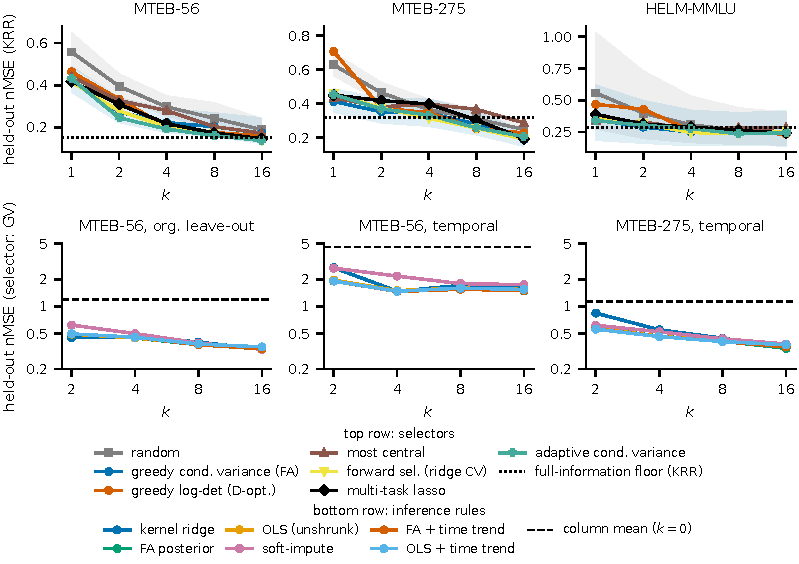
\includegraphics[width=\linewidth]{figA5_extra_baselines.pdf}
\caption{Top: kernel-ridge nMSE against $k$ for the base selectors and three further deployable selectors (bands: 95\% bootstrap CI over models for random and conditional variance only; dotted: full-information floor). Bottom: inference rules under organisation leave-out and temporal splits (conditional-variance set, log axis; dashed: column mean): kernel ridge, factor posterior, unshrunk OLS, soft-impute and the factor/OLS rule with a linear release-date trend.}
\label{fig:xbase}
\end{figure}
\begin{table}[h]
\caption{Selectors with kernel-ridge inference, random folds, same folds and repetitions as the base runs: nMSE $\pm$ half-width of the 95\% bootstrap CI over models.}
\label{tab:xsel}
\centering\scriptsize\setlength{\tabcolsep}{3pt}
\begin{tabular}{lrrrrr}
\toprule
 & \multicolumn{5}{c}{nMSE (KRR), number of benchmarks run $k$} \\
\cmidrule(lr){2-6}
selector & 1 & 2 & 4 & 8 & 16 \\
\midrule
\multicolumn{6}{l}{\emph{MTEB-56}} \\
random & 0.56\,{\scriptsize$\pm$0.08} & 0.39\,{\scriptsize$\pm$0.05} & 0.30\,{\scriptsize$\pm$0.05} & 0.24\,{\scriptsize$\pm$0.07} & 0.19\,{\scriptsize$\pm$0.05} \\
central & 0.44\,{\scriptsize$\pm$0.07} & 0.33\,{\scriptsize$\pm$0.05} & 0.28\,{\scriptsize$\pm$0.05} & 0.20\,{\scriptsize$\pm$0.05} & 0.17\,{\scriptsize$\pm$0.04} \\
GV & 0.42\,{\scriptsize$\pm$0.06} & 0.27\,{\scriptsize$\pm$0.06} & 0.22\,{\scriptsize$\pm$0.06} & 0.20\,{\scriptsize$\pm$0.06} & 0.17\,{\scriptsize$\pm$0.06} \\
D-opt & 0.46\,{\scriptsize$\pm$0.07} & 0.33\,{\scriptsize$\pm$0.05} & 0.20\,{\scriptsize$\pm$0.04} & 0.17\,{\scriptsize$\pm$0.04} & 0.16\,{\scriptsize$\pm$0.05} \\
adaptive GV & 0.43\,{\scriptsize$\pm$0.06} & 0.24\,{\scriptsize$\pm$0.04} & 0.19\,{\scriptsize$\pm$0.03} & 0.16\,{\scriptsize$\pm$0.03} & 0.14\,{\scriptsize$\pm$0.03} \\
fwd. ridge & 0.42\,{\scriptsize$\pm$0.06} & 0.28\,{\scriptsize$\pm$0.05} & 0.20\,{\scriptsize$\pm$0.03} & 0.17\,{\scriptsize$\pm$0.04} & 0.14\,{\scriptsize$\pm$0.04} \\
multi-task lasso & 0.42\,{\scriptsize$\pm$0.06} & 0.31\,{\scriptsize$\pm$0.06} & 0.22\,{\scriptsize$\pm$0.04} & 0.17\,{\scriptsize$\pm$0.04} & 0.15\,{\scriptsize$\pm$0.04} \\
\midrule
\multicolumn{6}{l}{\emph{MTEB-275}} \\
random & 0.63\,{\scriptsize$\pm$0.07} & 0.46\,{\scriptsize$\pm$0.06} & 0.36\,{\scriptsize$\pm$0.06} & 0.31\,{\scriptsize$\pm$0.06} & 0.25\,{\scriptsize$\pm$0.05} \\
central & 0.43\,{\scriptsize$\pm$0.08} & 0.38\,{\scriptsize$\pm$0.08} & 0.40\,{\scriptsize$\pm$0.09} & 0.37\,{\scriptsize$\pm$0.09} & 0.29\,{\scriptsize$\pm$0.07} \\
GV & 0.41\,{\scriptsize$\pm$0.07} & 0.35\,{\scriptsize$\pm$0.07} & 0.34\,{\scriptsize$\pm$0.08} & 0.28\,{\scriptsize$\pm$0.07} & 0.19\,{\scriptsize$\pm$0.04} \\
D-opt & 0.71\,{\scriptsize$\pm$0.11} & 0.37\,{\scriptsize$\pm$0.07} & 0.35\,{\scriptsize$\pm$0.09} & 0.25\,{\scriptsize$\pm$0.06} & 0.23\,{\scriptsize$\pm$0.06} \\
adaptive GV & 0.45\,{\scriptsize$\pm$0.08} & 0.37\,{\scriptsize$\pm$0.08} & 0.33\,{\scriptsize$\pm$0.09} & 0.26\,{\scriptsize$\pm$0.06} & 0.21\,{\scriptsize$\pm$0.04} \\
fwd. ridge & 0.46\,{\scriptsize$\pm$0.08} & 0.38\,{\scriptsize$\pm$0.08} & 0.31\,{\scriptsize$\pm$0.07} & 0.26\,{\scriptsize$\pm$0.06} & 0.19\,{\scriptsize$\pm$0.04} \\
multi-task lasso & 0.45\,{\scriptsize$\pm$0.07} & 0.42\,{\scriptsize$\pm$0.08} & 0.40\,{\scriptsize$\pm$0.09} & 0.30\,{\scriptsize$\pm$0.07} & 0.19\,{\scriptsize$\pm$0.04} \\
\midrule
\multicolumn{6}{l}{\emph{HELM-MMLU}} \\
random & 0.56\,{\scriptsize$\pm$0.38} & 0.40\,{\scriptsize$\pm$0.27} & 0.31\,{\scriptsize$\pm$0.18} & 0.26\,{\scriptsize$\pm$0.15} & 0.25\,{\scriptsize$\pm$0.13} \\
central & 0.34\,{\scriptsize$\pm$0.22} & 0.33\,{\scriptsize$\pm$0.23} & 0.27\,{\scriptsize$\pm$0.15} & 0.28\,{\scriptsize$\pm$0.16} & 0.28\,{\scriptsize$\pm$0.14} \\
GV & 0.35\,{\scriptsize$\pm$0.22} & 0.29\,{\scriptsize$\pm$0.17} & 0.25\,{\scriptsize$\pm$0.14} & 0.24\,{\scriptsize$\pm$0.13} & 0.25\,{\scriptsize$\pm$0.14} \\
D-opt & 0.47\,{\scriptsize$\pm$0.40} & 0.43\,{\scriptsize$\pm$0.37} & 0.26\,{\scriptsize$\pm$0.14} & 0.25\,{\scriptsize$\pm$0.14} & 0.23\,{\scriptsize$\pm$0.12} \\
adaptive GV & 0.34\,{\scriptsize$\pm$0.22} & 0.30\,{\scriptsize$\pm$0.19} & 0.28\,{\scriptsize$\pm$0.16} & 0.24\,{\scriptsize$\pm$0.12} & 0.24\,{\scriptsize$\pm$0.13} \\
fwd. ridge & 0.36\,{\scriptsize$\pm$0.23} & 0.31\,{\scriptsize$\pm$0.19} & 0.25\,{\scriptsize$\pm$0.13} & 0.24\,{\scriptsize$\pm$0.13} & 0.25\,{\scriptsize$\pm$0.14} \\
multi-task lasso & 0.39\,{\scriptsize$\pm$0.28} & 0.31\,{\scriptsize$\pm$0.20} & 0.29\,{\scriptsize$\pm$0.17} & 0.26\,{\scriptsize$\pm$0.15} & 0.24\,{\scriptsize$\pm$0.14} \\
\bottomrule
\end{tabular}

\end{table}
\begin{table}[h]
\caption{Differences in nMSE to random (left) and to conditional variance (right), CI from the bootstrap over strict families; $*$: CI excludes $0$. Against conditional variance the family-cluster CI excludes $0$ in $21$ of $75$ (selector $\times k$) cells: in $15$ conditional variance is better (central in $7$, log-det at $k=1$ on MTEB-275 by $0.29$, the rest by $\le0.09$), in $6$ the challenger is better by $\le0.04$.}
\label{tab:xselpaired}
\centering\scriptsize\setlength{\tabcolsep}{3pt}
\begin{tabular}{lrrrrrrrrrr}
\toprule
 & \multicolumn{5}{c}{$\Delta$ nMSE vs random} & \multicolumn{5}{c}{$\Delta$ nMSE vs GV} \\
\cmidrule(lr){2-6}\cmidrule(lr){7-11}
selector & 1 & 2 & 4 & 8 & 16 & 1 & 2 & 4 & 8 & 16 \\
\midrule
\multicolumn{11}{l}{\emph{MTEB-56}} \\
central & $-$0.12$^*$ & $-$0.07 & $-$0.02 & $-$0.04 & $-$0.02 & 0.02 & 0.06 & 0.06$^*$ & $-$0.00 & $-$0.01 \\
GV & $-$0.13$^*$ & $-$0.12$^*$ & $-$0.07$^*$ & $-$0.04$^*$ & $-$0.01 & -- & -- & -- & -- & -- \\
D-opt & $-$0.09$^*$ & $-$0.06$^*$ & $-$0.09$^*$ & $-$0.07$^*$ & $-$0.03$^*$ & 0.04 & 0.06 & $-$0.02 & $-$0.03 & $-$0.01 \\
adaptive GV & $-$0.13$^*$ & $-$0.15$^*$ & $-$0.11$^*$ & $-$0.08$^*$ & $-$0.05$^*$ & 0.01 & $-$0.03 & $-$0.03 & $-$0.04$^*$ & $-$0.04$^*$ \\
fwd. ridge & $-$0.14$^*$ & $-$0.12$^*$ & $-$0.09$^*$ & $-$0.07$^*$ & $-$0.05$^*$ & $-$0.01 & 0.01 & $-$0.02 & $-$0.03 & $-$0.04 \\
multi-task lasso & $-$0.14$^*$ & $-$0.09$^*$ & $-$0.08$^*$ & $-$0.07$^*$ & $-$0.04$^*$ & $-$0.01 & 0.04 & $-$0.01 & $-$0.03 & $-$0.03$^*$ \\
\midrule
\multicolumn{11}{l}{\emph{MTEB-275}} \\
central & $-$0.19$^*$ & $-$0.08$^*$ & 0.03 & 0.06 & 0.04$^*$ & 0.02$^*$ & 0.03 & 0.05 & 0.09$^*$ & 0.05$^*$ \\
GV & $-$0.22$^*$ & $-$0.11$^*$ & $-$0.02 & $-$0.03 & $-$0.02$^*$ & -- & -- & -- & -- & -- \\
D-opt & 0.08 & $-$0.09$^*$ & $-$0.02 & $-$0.06$^*$ & $-$0.02$^*$ & 0.29$^*$ & 0.02 & 0.00 & $-$0.03 & 0.01 \\
adaptive GV & $-$0.17$^*$ & $-$0.09$^*$ & $-$0.03 & $-$0.05$^*$ & $-$0.04$^*$ & 0.04$^*$ & 0.02 & $-$0.01 & $-$0.02 & $-$0.02 \\
fwd. ridge & $-$0.17$^*$ & $-$0.09$^*$ & $-$0.05$^*$ & $-$0.05$^*$ & $-$0.05$^*$ & 0.05$^*$ & 0.02 & $-$0.03$^*$ & $-$0.02 & $-$0.02$^*$ \\
multi-task lasso & $-$0.18$^*$ & $-$0.05 & 0.03 & $-$0.01 & $-$0.03$^*$ & 0.04 & 0.07$^*$ & 0.05 & 0.02 & $-$0.01 \\
\midrule
\multicolumn{11}{l}{\emph{HELM-MMLU}} \\
central & $-$0.22$^*$ & $-$0.07$^*$ & $-$0.03$^*$ & 0.02 & 0.03$^*$ & $-$0.01 & 0.04 & 0.02$^*$ & 0.04$^*$ & 0.04$^*$ \\
GV & $-$0.21$^*$ & $-$0.11$^*$ & $-$0.06$^*$ & $-$0.02$^*$ & $-$0.00 & -- & -- & -- & -- & -- \\
D-opt & $-$0.09$^*$ & 0.03 & $-$0.04$^*$ & $-$0.02$^*$ & $-$0.02$^*$ & 0.12 & 0.14 & 0.01$^*$ & 0.00 & $-$0.01 \\
adaptive GV & $-$0.22$^*$ & $-$0.10$^*$ & $-$0.03$^*$ & $-$0.03$^*$ & $-$0.01$^*$ & $-$0.01$^*$ & 0.01 & 0.03$^*$ & $-$0.01 & $-$0.01 \\
fwd. ridge & $-$0.20$^*$ & $-$0.08$^*$ & $-$0.06$^*$ & $-$0.03$^*$ & 0.00 & 0.01 & 0.03$^*$ & $-$0.00 & $-$0.01 & 0.01 \\
multi-task lasso & $-$0.17$^*$ & $-$0.09$^*$ & $-$0.02$^*$ & $-$0.00 & $-$0.01 & 0.04 & 0.02 & 0.04$^*$ & 0.02 & $-$0.01 \\
\bottomrule
\end{tabular}

\end{table}
\begin{table}[h]
\caption{Inference rules under random folds with random and conditional-variance selection: kernel ridge, factor posterior with CV rank, fixed rank 1 and 2, unshrunk OLS and soft-impute; nMSE $\pm$ half-width of the 95\% CI over models.}
\label{tab:xrules}
\centering\scriptsize\setlength{\tabcolsep}{3pt}
\begin{tabular}{lrrrrrrrr}
\toprule
 & \multicolumn{4}{c}{random selection} & \multicolumn{4}{c}{greedy cond. variance} \\
\cmidrule(lr){2-5}\cmidrule(lr){6-9}
rule & 2 & 4 & 8 & 16 & 2 & 4 & 8 & 16 \\
\midrule
\multicolumn{9}{l}{\emph{MTEB-56}} \\
kernel ridge & 0.39{\tiny$\pm$0.05} & 0.30{\tiny$\pm$0.05} & 0.24{\tiny$\pm$0.07} & 0.19{\tiny$\pm$0.05} & 0.27{\tiny$\pm$0.06} & 0.22{\tiny$\pm$0.06} & 0.20{\tiny$\pm$0.06} & 0.17{\tiny$\pm$0.06} \\
FA (CV rank) & 0.48{\tiny$\pm$0.06} & 0.36{\tiny$\pm$0.05} & 0.29{\tiny$\pm$0.06} & 0.23{\tiny$\pm$0.04} & 0.36{\tiny$\pm$0.06} & 0.28{\tiny$\pm$0.06} & 0.24{\tiny$\pm$0.06} & 0.22{\tiny$\pm$0.06} \\
FA, $r=1$ & 0.54{\tiny$\pm$0.07} & 0.48{\tiny$\pm$0.07} & 0.43{\tiny$\pm$0.06} & 0.41{\tiny$\pm$0.06} & 0.46{\tiny$\pm$0.07} & 0.42{\tiny$\pm$0.06} & 0.40{\tiny$\pm$0.06} & 0.38{\tiny$\pm$0.06} \\
FA, $r=2$ & 0.49{\tiny$\pm$0.06} & 0.39{\tiny$\pm$0.06} & 0.33{\tiny$\pm$0.05} & 0.30{\tiny$\pm$0.05} & 0.37{\tiny$\pm$0.06} & 0.33{\tiny$\pm$0.05} & 0.31{\tiny$\pm$0.05} & 0.29{\tiny$\pm$0.05} \\
OLS & 0.48{\tiny$\pm$0.06} & 0.36{\tiny$\pm$0.05} & 0.30{\tiny$\pm$0.08} & 0.25{\tiny$\pm$0.07} & 0.36{\tiny$\pm$0.06} & 0.28{\tiny$\pm$0.06} & 0.24{\tiny$\pm$0.06} & 0.21{\tiny$\pm$0.06} \\
soft-impute & 0.59{\tiny$\pm$0.09} & 0.45{\tiny$\pm$0.07} & 0.34{\tiny$\pm$0.05} & 0.27{\tiny$\pm$0.04} & 0.50{\tiny$\pm$0.09} & 0.37{\tiny$\pm$0.05} & 0.31{\tiny$\pm$0.04} & 0.26{\tiny$\pm$0.05} \\
\midrule
\multicolumn{9}{l}{\emph{MTEB-275}} \\
kernel ridge & 0.46{\tiny$\pm$0.06} & 0.36{\tiny$\pm$0.06} & 0.31{\tiny$\pm$0.06} & 0.25{\tiny$\pm$0.05} & 0.35{\tiny$\pm$0.07} & 0.34{\tiny$\pm$0.08} & 0.28{\tiny$\pm$0.07} & 0.19{\tiny$\pm$0.04} \\
FA (CV rank) & 0.54{\tiny$\pm$0.06} & 0.42{\tiny$\pm$0.05} & 0.34{\tiny$\pm$0.05} & 0.28{\tiny$\pm$0.04} & 0.42{\tiny$\pm$0.07} & 0.34{\tiny$\pm$0.06} & 0.29{\tiny$\pm$0.06} & 0.21{\tiny$\pm$0.04} \\
FA, $r=1$ & 0.63{\tiny$\pm$0.06} & 0.56{\tiny$\pm$0.06} & 0.52{\tiny$\pm$0.05} & 0.50{\tiny$\pm$0.05} & 0.54{\tiny$\pm$0.07} & 0.50{\tiny$\pm$0.06} & 0.49{\tiny$\pm$0.05} & 0.47{\tiny$\pm$0.05} \\
FA, $r=2$ & 0.55{\tiny$\pm$0.06} & 0.44{\tiny$\pm$0.06} & 0.38{\tiny$\pm$0.05} & 0.35{\tiny$\pm$0.05} & 0.41{\tiny$\pm$0.07} & 0.36{\tiny$\pm$0.06} & 0.34{\tiny$\pm$0.05} & 0.29{\tiny$\pm$0.04} \\
OLS & 0.54{\tiny$\pm$0.06} & 0.42{\tiny$\pm$0.05} & 0.34{\tiny$\pm$0.05} & 0.29{\tiny$\pm$0.05} & 0.42{\tiny$\pm$0.07} & 0.34{\tiny$\pm$0.06} & 0.29{\tiny$\pm$0.06} & 0.21{\tiny$\pm$0.04} \\
soft-impute & 0.64{\tiny$\pm$0.07} & 0.50{\tiny$\pm$0.06} & 0.40{\tiny$\pm$0.05} & 0.32{\tiny$\pm$0.04} & 0.57{\tiny$\pm$0.07} & 0.45{\tiny$\pm$0.06} & 0.35{\tiny$\pm$0.05} & 0.26{\tiny$\pm$0.03} \\
\midrule
\multicolumn{9}{l}{\emph{HELM-MMLU}} \\
kernel ridge & 0.40{\tiny$\pm$0.27} & 0.31{\tiny$\pm$0.18} & 0.26{\tiny$\pm$0.15} & 0.25{\tiny$\pm$0.13} & 0.29{\tiny$\pm$0.17} & 0.25{\tiny$\pm$0.14} & 0.24{\tiny$\pm$0.13} & 0.25{\tiny$\pm$0.14} \\
FA (CV rank) & 0.43{\tiny$\pm$0.27} & 0.33{\tiny$\pm$0.18} & 0.27{\tiny$\pm$0.14} & 0.23{\tiny$\pm$0.11} & 0.31{\tiny$\pm$0.16} & 0.27{\tiny$\pm$0.14} & 0.25{\tiny$\pm$0.13} & 0.23{\tiny$\pm$0.12} \\
FA, $r=1$ & 0.46{\tiny$\pm$0.31} & 0.40{\tiny$\pm$0.26} & 0.36{\tiny$\pm$0.24} & 0.34{\tiny$\pm$0.23} & 0.38{\tiny$\pm$0.23} & 0.37{\tiny$\pm$0.25} & 0.36{\tiny$\pm$0.23} & 0.35{\tiny$\pm$0.23} \\
FA, $r=2$ & 0.43{\tiny$\pm$0.27} & 0.32{\tiny$\pm$0.18} & 0.27{\tiny$\pm$0.15} & 0.24{\tiny$\pm$0.12} & 0.30{\tiny$\pm$0.16} & 0.28{\tiny$\pm$0.16} & 0.27{\tiny$\pm$0.15} & 0.25{\tiny$\pm$0.14} \\
OLS & 0.43{\tiny$\pm$0.27} & 0.33{\tiny$\pm$0.18} & 0.28{\tiny$\pm$0.15} & 0.28{\tiny$\pm$0.14} & 0.30{\tiny$\pm$0.16} & 0.27{\tiny$\pm$0.15} & 0.26{\tiny$\pm$0.14} & 0.27{\tiny$\pm$0.16} \\
soft-impute & 0.55{\tiny$\pm$0.35} & 0.41{\tiny$\pm$0.26} & 0.33{\tiny$\pm$0.21} & 0.27{\tiny$\pm$0.16} & 0.52{\tiny$\pm$0.39} & 0.37{\tiny$\pm$0.22} & 0.30{\tiny$\pm$0.17} & 0.26{\tiny$\pm$0.15} \\
\bottomrule
\end{tabular}

\end{table}
\paragraph{Leverage and QR at fixed rank.} With the rank of the leverage and QR criteria fixed at $3$ rather than chosen by cross-validation ($8$--$16$), both reach $\nmse\le0.5$ at $k=3$ (kernel ridge) against $4$--$6$ at the cross-validated rank, and $\nmse\le0.25$ at $k=12$ against $12$--$16$ (\texttt{kstar\_d56\_selrank2.csv}); at the cross-validated rank their first eight picks have mean pairwise $|\mathrm{corr}|$ $0.43$--$0.49$ (random $0.62$, conditional variance $0.59$, log-det $0.67$) and mean uniqueness $0.24$--$0.29$ (conditional variance and random $0.09$--$0.10$, log-det $0.01$) (\texttt{lev\_diag\_mteb\_dense56.csv}). The failure of these criteria at small $k$ is thus mostly a rank mis-specification that selects task-specific (noisy) tasks, not a redundant cluster.
\paragraph{Temporal drift and the out-of-range check.} Fig.~\ref{fig:xbase} (bottom) and Table~\ref{tab:drift} show the rules on the single temporal fold and under rolling origin, Table~\ref{tab:ood} the detector. The detector scores the $k$ revealed scores of a new model by their squared Mahalanobis distance under the shrunk empirical covariance of the training models and flags it above the $95\%$ $\chi^2$ quantile; it is a check on the input, not a calibrated predictor of error. In a rolling-origin evaluation (four cutoffs at $55$--$85\%$ of dated models, next $15\%$ as test) the factor posterior with conditional-variance selection gives $0.96/0.91/0.87/0.74$ at $k=2/4/8/16$ on MTEB-56 against $2.18$ for the mean and $2.03$ for the mean with trend; on MTEB-275 $0.58/0.48/0.45/0.39$ against $1.28$ and $1.37$ (\texttt{extra\_temporal\_summary.csv}).
\begin{table}[h]
\caption{Out-of-range detector (selector: conditional variance; flag: squared Mahalanobis distance of the $k$ revealed scores above the $95\%$ $\chi^2$ quantile of the shrunk training covariance). AUC: of the distance for the worst tercile of the model's own nMSE (kernel ridge); mean nMSE of flagged and unflagged models with 95\% bootstrap CI over models (n/a: fewer than $3$ flagged).}
\label{tab:ood}
\centering\scriptsize\setlength{\tabcolsep}{3pt}
\begin{tabular}{lrrrcc}
\toprule
matrix, split & $k$ & flagged & AUC & nMSE flagged & nMSE unflagged \\
\midrule
MTEB-56, random folds & 4 & 12/152 & 0.66 & 0.71 {\scriptsize[0.23, 1.43]} & 0.18 {\scriptsize[0.15, 0.21]} \\
 & 8 & 11/152 & 0.82 & 0.83 {\scriptsize[0.32, 1.60]} & 0.15 {\scriptsize[0.13, 0.18]} \\
 & 16 & 10/148 & 0.86 & 0.94 {\scriptsize[0.34, 1.77]} & 0.12 {\scriptsize[0.10, 0.14]} \\
\midrule
MTEB-56, org.\ leave-out & 4 & 14/152 & 0.79 & 2.25 {\scriptsize[0.97, 4.13]} & 0.28 {\scriptsize[0.23, 0.34]} \\
 & 8 & 12/152 & 0.80 & 2.44 {\scriptsize[1.12, 4.14]} & 0.22 {\scriptsize[0.19, 0.26]} \\
 & 16 & 22/150 & 0.88 & 1.31 {\scriptsize[0.79, 2.14]} & 0.17 {\scriptsize[0.15, 0.20]} \\
\midrule
MTEB-56, family leave-out & 4 & 7/152 & 0.73 & 2.01 {\scriptsize[0.63, 4.88]} & 0.30 {\scriptsize[0.26, 0.34]} \\
 & 8 & 15/152 & 0.84 & 1.19 {\scriptsize[0.55, 2.27]} & 0.23 {\scriptsize[0.20, 0.25]} \\
 & 16 & 21/148 & 0.84 & 0.93 {\scriptsize[0.47, 1.83]} & 0.19 {\scriptsize[0.16, 0.21]} \\
\midrule
MTEB-56, temporal & 4 & 14/31 & 0.93 & 2.41 {\scriptsize[1.66, 3.18]} & 0.73 {\scriptsize[0.30, 1.46]} \\
 & 8 & 12/31 & 0.96 & 3.62 {\scriptsize[2.81, 4.32]} & 0.56 {\scriptsize[0.37, 0.78]} \\
 & 16 & 14/29 & 0.89 & 2.52 {\scriptsize[1.65, 3.32]} & 0.75 {\scriptsize[0.30, 1.33]} \\
\midrule
MTEB-275, random folds & 4 & 1/133 & 0.72 & 2.13 {\scriptsize[n/a]} & 0.33 {\scriptsize[0.26, 0.41]} \\
 & 8 & 7/133 & 0.85 & 1.48 {\scriptsize[0.69, 2.21]} & 0.21 {\scriptsize[0.18, 0.26]} \\
 & 16 & 5/112 & 0.84 & 0.67 {\scriptsize[0.16, 1.32]} & 0.17 {\scriptsize[0.13, 0.20]} \\
\midrule
MTEB-275, org.\ leave-out & 4 & 11/133 & 0.74 & 2.01 {\scriptsize[1.39, 2.76]} & 0.32 {\scriptsize[0.28, 0.37]} \\
 & 8 & 12/133 & 0.83 & 1.36 {\scriptsize[0.97, 1.95]} & 0.27 {\scriptsize[0.23, 0.32]} \\
 & 16 & 13/113 & 0.90 & 0.70 {\scriptsize[0.58, 0.80]} & 0.20 {\scriptsize[0.17, 0.23]} \\
\midrule
MTEB-275, temporal & 4 & 1/27 & 0.70 & 0.58 {\scriptsize[n/a]} & 0.55 {\scriptsize[0.43, 0.71]} \\
 & 8 & 2/27 & 0.68 & 1.33 {\scriptsize[n/a]} & 0.37 {\scriptsize[0.29, 0.45]} \\
 & 16 & 3/15 & 0.96 & 0.65 {\scriptsize[0.35, 0.97]} & 0.27 {\scriptsize[0.18, 0.38]} \\
\bottomrule
\end{tabular}

\end{table}
\begin{table}[h]
\caption{Temporal drift on MTEB-56 and MTEB-275 (dated models only). (a) Single temporal fold (train: earliest $4/5$, test: newest $\approx1/5$; conditional-variance selection): nMSE $\pm$ half-width of the 95\% CI over models for six inference rules, including a linear release-date trend added to the factor and OLS rules; the column mean ($k=0$) is in the last row of the block. (b) Rolling origin (cutoffs at $55,65,75,85\%$ of the dated models, the next $15\%$ as test, pooled over the four origins): random against conditional-variance selection, with the column mean and the column mean plus trend at $k=0$.}
\label{tab:drift}
\centering\tiny\setlength{\tabcolsep}{2pt}
\begin{tabular}{lrrrrrrrr}
\toprule
 & \multicolumn{4}{c}{MTEB-56} & \multicolumn{4}{c}{MTEB-275} \\
\cmidrule(lr){2-5}\cmidrule(lr){6-9}
rule & 2 & 4 & 8 & 16 & 2 & 4 & 8 & 16 \\
\midrule
\multicolumn{9}{l}{\emph{(a) single temporal fold, selector GV, test = newest $\approx$20\% of dated models}} \\
FA & 1.96{\tiny$\pm$0.71} & 1.50{\tiny$\pm$0.54} & 1.56{\tiny$\pm$0.53} & 1.49{\tiny$\pm$0.55} & 0.57{\tiny$\pm$0.11} & 0.47{\tiny$\pm$0.08} & 0.41{\tiny$\pm$0.07} & 0.34{\tiny$\pm$0.10} \\
KRR & 2.69{\tiny$\pm$0.92} & 1.47{\tiny$\pm$0.55} & 1.71{\tiny$\pm$0.58} & 1.58{\tiny$\pm$0.56} & 0.84{\tiny$\pm$0.25} & 0.55{\tiny$\pm$0.14} & 0.44{\tiny$\pm$0.12} & 0.35{\tiny$\pm$0.12} \\
OLS (unshrunk) & 1.96{\tiny$\pm$0.71} & 1.49{\tiny$\pm$0.53} & 1.60{\tiny$\pm$0.53} & 1.54{\tiny$\pm$0.56} & 0.57{\tiny$\pm$0.11} & 0.46{\tiny$\pm$0.08} & 0.41{\tiny$\pm$0.07} & 0.37{\tiny$\pm$0.13} \\
soft-impute & 2.66{\tiny$\pm$0.96} & 2.17{\tiny$\pm$0.78} & 1.79{\tiny$\pm$0.59} & 1.74{\tiny$\pm$0.62} & 0.62{\tiny$\pm$0.11} & 0.52{\tiny$\pm$0.08} & 0.44{\tiny$\pm$0.07} & 0.38{\tiny$\pm$0.09} \\
FA + trend & 1.91{\tiny$\pm$0.68} & 1.46{\tiny$\pm$0.53} & 1.55{\tiny$\pm$0.53} & 1.50{\tiny$\pm$0.56} & 0.56{\tiny$\pm$0.11} & 0.46{\tiny$\pm$0.07} & 0.41{\tiny$\pm$0.07} & 0.35{\tiny$\pm$0.10} \\
OLS + trend & 1.91{\tiny$\pm$0.68} & 1.47{\tiny$\pm$0.53} & 1.59{\tiny$\pm$0.53} & 1.54{\tiny$\pm$0.56} & 0.56{\tiny$\pm$0.11} & 0.46{\tiny$\pm$0.07} & 0.41{\tiny$\pm$0.07} & 0.37{\tiny$\pm$0.12} \\
avg.-score regression & 2.13{\tiny$\pm$0.73} & 2.16{\tiny$\pm$0.72} & 1.81{\tiny$\pm$0.56} & 1.98{\tiny$\pm$0.64} & 0.58{\tiny$\pm$0.11} & 0.54{\tiny$\pm$0.09} & 0.51{\tiny$\pm$0.08} & 0.55{\tiny$\pm$0.14} \\
column mean ($k=0$) & \multicolumn{4}{c}{4.57} & \multicolumn{4}{c}{1.14} \\
\midrule
\multicolumn{9}{l}{\emph{(b) rolling origin (cutoffs 55/65/75/85\%, next 15\% as test), pooled}} \\
FA, random & 1.25{\tiny$\pm$0.34} & 1.04{\tiny$\pm$0.28} & 0.84{\tiny$\pm$0.25} & 0.74{\tiny$\pm$0.23} & 0.73{\tiny$\pm$0.10} & 0.59{\tiny$\pm$0.08} & 0.49{\tiny$\pm$0.08} & 0.43{\tiny$\pm$0.07} \\
KRR, random & 1.18{\tiny$\pm$0.28} & 0.99{\tiny$\pm$0.24} & 0.88{\tiny$\pm$0.23} & 0.85{\tiny$\pm$0.23} & 0.69{\tiny$\pm$0.10} & 0.58{\tiny$\pm$0.10} & 0.48{\tiny$\pm$0.09} & 0.42{\tiny$\pm$0.08} \\
soft-impute, random & 1.38{\tiny$\pm$0.38} & 1.12{\tiny$\pm$0.32} & 0.92{\tiny$\pm$0.25} & 0.78{\tiny$\pm$0.21} & 0.83{\tiny$\pm$0.11} & 0.65{\tiny$\pm$0.09} & 0.53{\tiny$\pm$0.07} & 0.44{\tiny$\pm$0.06} \\
FA + trend, random & 1.29{\tiny$\pm$0.32} & 1.08{\tiny$\pm$0.28} & 0.86{\tiny$\pm$0.25} & 0.76{\tiny$\pm$0.25} & 0.79{\tiny$\pm$0.11} & 0.62{\tiny$\pm$0.09} & 0.50{\tiny$\pm$0.08} & 0.44{\tiny$\pm$0.08} \\
FA, GV & 0.96{\tiny$\pm$0.31} & 0.91{\tiny$\pm$0.42} & 0.87{\tiny$\pm$0.44} & 0.74{\tiny$\pm$0.43} & 0.58{\tiny$\pm$0.09} & 0.48{\tiny$\pm$0.08} & 0.45{\tiny$\pm$0.10} & 0.39{\tiny$\pm$0.11} \\
KRR, GV & 1.15{\tiny$\pm$0.28} & 1.03{\tiny$\pm$0.41} & 0.94{\tiny$\pm$0.39} & 0.93{\tiny$\pm$0.42} & 0.56{\tiny$\pm$0.12} & 0.51{\tiny$\pm$0.11} & 0.46{\tiny$\pm$0.12} & 0.38{\tiny$\pm$0.11} \\
soft-impute, GV & 1.24{\tiny$\pm$0.32} & 1.02{\tiny$\pm$0.34} & 0.86{\tiny$\pm$0.27} & 0.71{\tiny$\pm$0.23} & 0.70{\tiny$\pm$0.10} & 0.55{\tiny$\pm$0.08} & 0.49{\tiny$\pm$0.07} & 0.40{\tiny$\pm$0.06} \\
FA + trend, GV & 0.98{\tiny$\pm$0.29} & 0.93{\tiny$\pm$0.49} & 0.90{\tiny$\pm$0.46} & 0.78{\tiny$\pm$0.47} & 0.59{\tiny$\pm$0.09} & 0.49{\tiny$\pm$0.09} & 0.47{\tiny$\pm$0.11} & 0.40{\tiny$\pm$0.11} \\
column mean ($k=0$) & \multicolumn{4}{c}{2.18} & \multicolumn{4}{c}{1.28} \\
column mean + trend ($k=0$) & \multicolumn{4}{c}{2.03} & \multicolumn{4}{c}{1.37} \\
\bottomrule
\end{tabular}

\end{table}
\paragraph{Sparse matrix.} \texttt{mteb-sparse} has $479$ models $\times$ $472$ tasks with $30.2\%$ of the cells observed ($2$ repetitions of $10$-fold CV, about $1.2$ h each); its description in \texttt{sparse\_population.csv} shows who the dense blocks leave out: the raw matrix has $536$ models and $1289$ tasks ($12\%$ observed), \texttt{mteb-dense56} keeps $28\%$ of the models, $4\%$ of the tasks and $10\%$ of the observed cells, \texttt{mteb-sparse} $89\%$, $37\%$ and $80\%$. A held-out model reveals the first $k$ benchmarks of the selector's ordering for which it has scores and models with fewer than $k$ scores are skipped for that $k$, so large-$k$ points rest on fewer models and $k=48$ on a small subset; targets are the observed cells of the fixed target benchmarks. Column-mean nMSE is $1.06$; the full-information floors are $0.18$ (factor posterior, 95\% CI $0.15$--$0.20$), $0.23$ (kNN) and $0.43$ (kernel ridge, ridge: these rules complete the matrix by mean imputation, so $G$ against their own floor is lenient and the floor of the best rule is the honest reference). nMSE with conditional variance / random selection ($k=2/4/8/16/32$): factor posterior $0.59/0.45/0.37/0.30/0.22$ and $0.65/0.52/0.42/0.33/0.26$; kernel ridge $0.44/0.35/0.34/0.29/0.22$ and $0.53/0.45/0.36/0.32/0.30$. Paired differences to random (model-level CI): conditional variance with the factor posterior $-0.047/-0.070/-0.083/-0.059/-0.024/+0.002$ at $k=1/2/4/8/16/32$ (CI excludes $0$ up to $k=8$); log-det is worse than random for $k\le4$ ($+0.18$, $+0.17$, $+0.045$ at $k=1,2,4$) and indistinguishable from $k=8$; central is better at $k=1,2$ ($-0.135$, $-0.047$) and worse from $k=4$ ($+0.039$ to $+0.137$). $k^\star(G\ge0.8)$ with the factor posterior (\texttt{kstar\_table.csv}): $16$ for conditional variance and random, $24$ for log-det; at $g=0.9$: $32$, $48$, $24$. With kernel ridge the criterion is reached at $2$ (conditional variance), $4$ (log-det), $3$ (random) against its own floor and at $12$, $12$, $10$ against the best floor. In the cluster-bootstrap run ($1000$ resamples, \texttt{cluster\_kstar\_B\_mteb\_sparse.csv}) the factor-posterior $k^\star$ is $16$ for conditional variance, log-det and random under model resampling and $16$, $24$, $16$ under family resampling, with point values $12$, $12$, $16$ (the $24$ for log-det in \texttt{kstar\_table.csv} against $16$ here shows the lower-bound rule grazing the criterion). The train-only Bayes curve is \emph{above} the cross-validated error at $k\le4$ (conditional variance: $0.67$, $0.53$ against $0.59$, $0.45$) and below it from $k=16$ ($0.17$ against $0.30$), so the model-implied curve does not bound the error on this matrix. Two repetitions only.

\section{Reproduction notes}
\label{app:repro}
The repository root \texttt{README.md} gives the complete notes; this section lists what a reader needs to check the paper.
\paragraph{Data pins.} MTEB results at commit \texttt{6dabbcc6\ldots}; Open LLM Leaderboard \texttt{open-llm-leaderboard/contents} at \texttt{9c09a7ca\ldots}; HELM Lite and HELM MMLU v1.13.0; LiveBench \texttt{model\_judgment} at \texttt{9704e5da\ldots} (full SHAs in \texttt{README.md}). \texttt{code/fetch\_data.sh} fetches them ($\approx3.3$~GB); the HELM Lite matrix with $91\times28$ entries is built from the pinned HELM Lite v1.13.0 export by \texttt{code/build\_helm\_ext.py}. The pinned Open LLM Leaderboard export has six aggregate benchmarks (no per-subtask scores) and the pinned LiveBench export seven task-level scores; per-subtask leaderboard details are not part of the pinned material and were not fetched, so no larger generative-LLM matrix than HELM Lite ($91\times28$) and HELM-MMLU ($79\times57$) could be built.
\paragraph{Software and hardware.} Python 3.11.2, numpy 2.4.6, scipy 1.17.1, pandas 3.0.6, pyarrow 26.0.0 (\texttt{code/requirements.txt}); CPU only. Wall-clock times on a shared host: MTEB-56 sweeps $20$--$55$ min, MTEB-275/357 sweeps $1.5$--$3$ h, small-$N$ matrices minutes; CPU-hours were not metered.
\paragraph{Seeds.} \texttt{--seed 0}; repetition $i$ uses \texttt{default\_rng(1000*seed+$i$)} and factor-analysis initialisation seed $i$; $3$ repetitions of 10-fold CV on MTEB-56, $2$ on MTEB-275/357, $5$ on HELM-MMLU; $10$ random-selector draws per fold ($5$ for the Open LLM Leaderboard). Bootstrap: $500$ resamples.
\paragraph{Script to table or figure.} \texttt{code/run\_cv.py} (one run per command in \texttt{code/launch\_sweeps.sh}) $\to$ \texttt{results/raw} $\to$ \texttt{code/analyze.py} $\to$ \texttt{results/summary}, \texttt{results/theory}; \texttt{code/figtab/make\_all.sh} writes every figure and table from those CSVs (map in \texttt{figures/PROVENANCE.md}). Every run has a launch line: \texttt{code/launch\_primary.sh} (\texttt{B\_*}, \texttt{A\_*}, \texttt{F\_*}), \texttt{launch\_sweeps.sh}, \texttt{launch\_syn.sh} and \texttt{launch\_review.sh} (cluster bootstrap, extra selectors and rules, shift rules, detector); \texttt{LOCAL=1 bash code/launch\_primary.sh} runs them sequentially in plain Python and \texttt{bash code/check.sh} regenerates one small run in about 12 s and compares it with \texttt{results/check/expected.csv}. The raw per-model tables ($450$~MB compressed) are the release \texttt{raw-results-1} of the experiment repository.
\paragraph{Not finished.} Every primary run listed above finished. Per-run wall-clock was not logged. The raw per-model tables are a release asset (\texttt{raw-results-1}, sparse run included), not versioned in the repository.
\paragraph{Forbidden-content log.} The task excludes the published paper on this question and anything citing it. No search made for this study (context review, reference verification) returned such a work; none was read or used. A reviewer pointed to two works on low-rank factors and adaptive calibration for LLM evaluation; because they may fall under the exclusion they were not read or cited.

\section{Voluntary self-audit (not an ICLR form)}
\label{app:audit}
ICLR 2027 has no mandatory checklist; we answer the following items for checkability.
\begin{enumerate}\itemsep0pt
\item \emph{Claims match the evidence and its scope.} Yes: Sections~\ref{sec:exp}, \ref{sec:disc}; scope is embedding-model matrices (MTEB) plus five small generative-LLM matrices and one sparse MTEB matrix, random-fold and shift splits.
\item \emph{Limitations and failure cases.} Yes: Section~\ref{sec:disc} (temporal extrapolation, small $M$, sparsity, small-$N$ leaderboards, cost-aware instability).
\item \emph{Theory: assumptions, proofs, check.} Yes: Appendix~\ref{app:theory}; checked on synthetic and real matrices (Fig.~\ref{fig:theory}).
\item \emph{Setting specified.} Yes: Section~\ref{sec:protocol}, Appendix~\ref{app:repro}.
\item \emph{Uncertainty.} Yes: 95\% bootstrap over held-out models for every curve and paired difference; shift splits have few held-out models and are marked.
\item \emph{Compute.} Yes: CPU only, times in Appendix~\ref{app:repro}.
\item \emph{Authorship accountability (ICLR AI policy).} No: no human author exists and none reviewed the work; see the AI-use statement.
\item \emph{Code and data.} Yes: scripts, versions, commands, map; licences: several source leaderboards declare none (ethics statement).
\item \emph{Every number traces to a script.} Yes: \texttt{results/summary}, \texttt{results/theory}, \texttt{figures/PROVENANCE.md}.
\item \emph{Citations.} Yes: all entries were checked against public metadata; forbidden-content log in Appendix~\ref{app:repro}.
\item \emph{Failed and unfinished runs reported.} Yes: Section~\ref{sec:data}, Appendix~\ref{app:repro}.
\end{enumerate}
